\section{Search for heavy \(Y \rightarrow XX\)}
\label{sec:org96b6be0}
\label{sec:Search_Y_to_XX}
\subsection{The \(Y \rightarrow XX\)channel}
\label{sec:org0fd1492}
\label{sec:The_YtoXX_channel}
The \(Y \rightarrow XX\) dataset is composed of simulated events that represent the generic process of a resonance Y decaying into an XX pair, in the mass range between 100 and 300 GeV. The background consists of 50,839 events, while the signal comprises 5,946 events. The particular set is made up of miscellaneous pre-existing Monte Carlo (MC) samples, and the selected events contain only leptonic final states (one lepton and one antilepton of the same flavor). For the purpose of this study, only generator-level events were used, and given that we are not interested in any particular process, but rather in the most general case, no kinematic constraints were placed in the event selection. It should be noted that despite the fact that the parent MC samples contain lepton pairs in the final states, the resulting set can represent any diobject production in the selected mass range. The following table summarizes the features of the dataset in question:

\begin{table}[h!]
\centering
\begin{tabular}{ |p{3cm}|p{10cm}|  }
 \hline
Feature & Description \\
 \hline
$Pt_{1}$ &  The transverse momentum of the first particle in the XX pair \\
 \hline
$\eta_{1}$ &  The psudorapidity of the first particle in the XX pair \\
 \hline
$\phi_{1}$ &   azimuth angle of the first particle in the XX pair \\
 \hline
$Pt_{2}$ &  The transverse momentum of the second particle in the XX pair \\
 \hline
$\eta_{2}$ &  The psudorapidity of the second particle in the XX pair \\
 \hline
$\phi_{2}$ &   azimuth angle of the second particle in the XX pair \\
 \hline
\end{tabular}
\caption{Summary of the data set features }
\label{table:DataSetFeatures}
\end{table}

The mass spectrum for the \(Y \rightarrow XX\) decay, can be seen in figure \ref{fig:diX}

\begin{figure}[h]
\centering
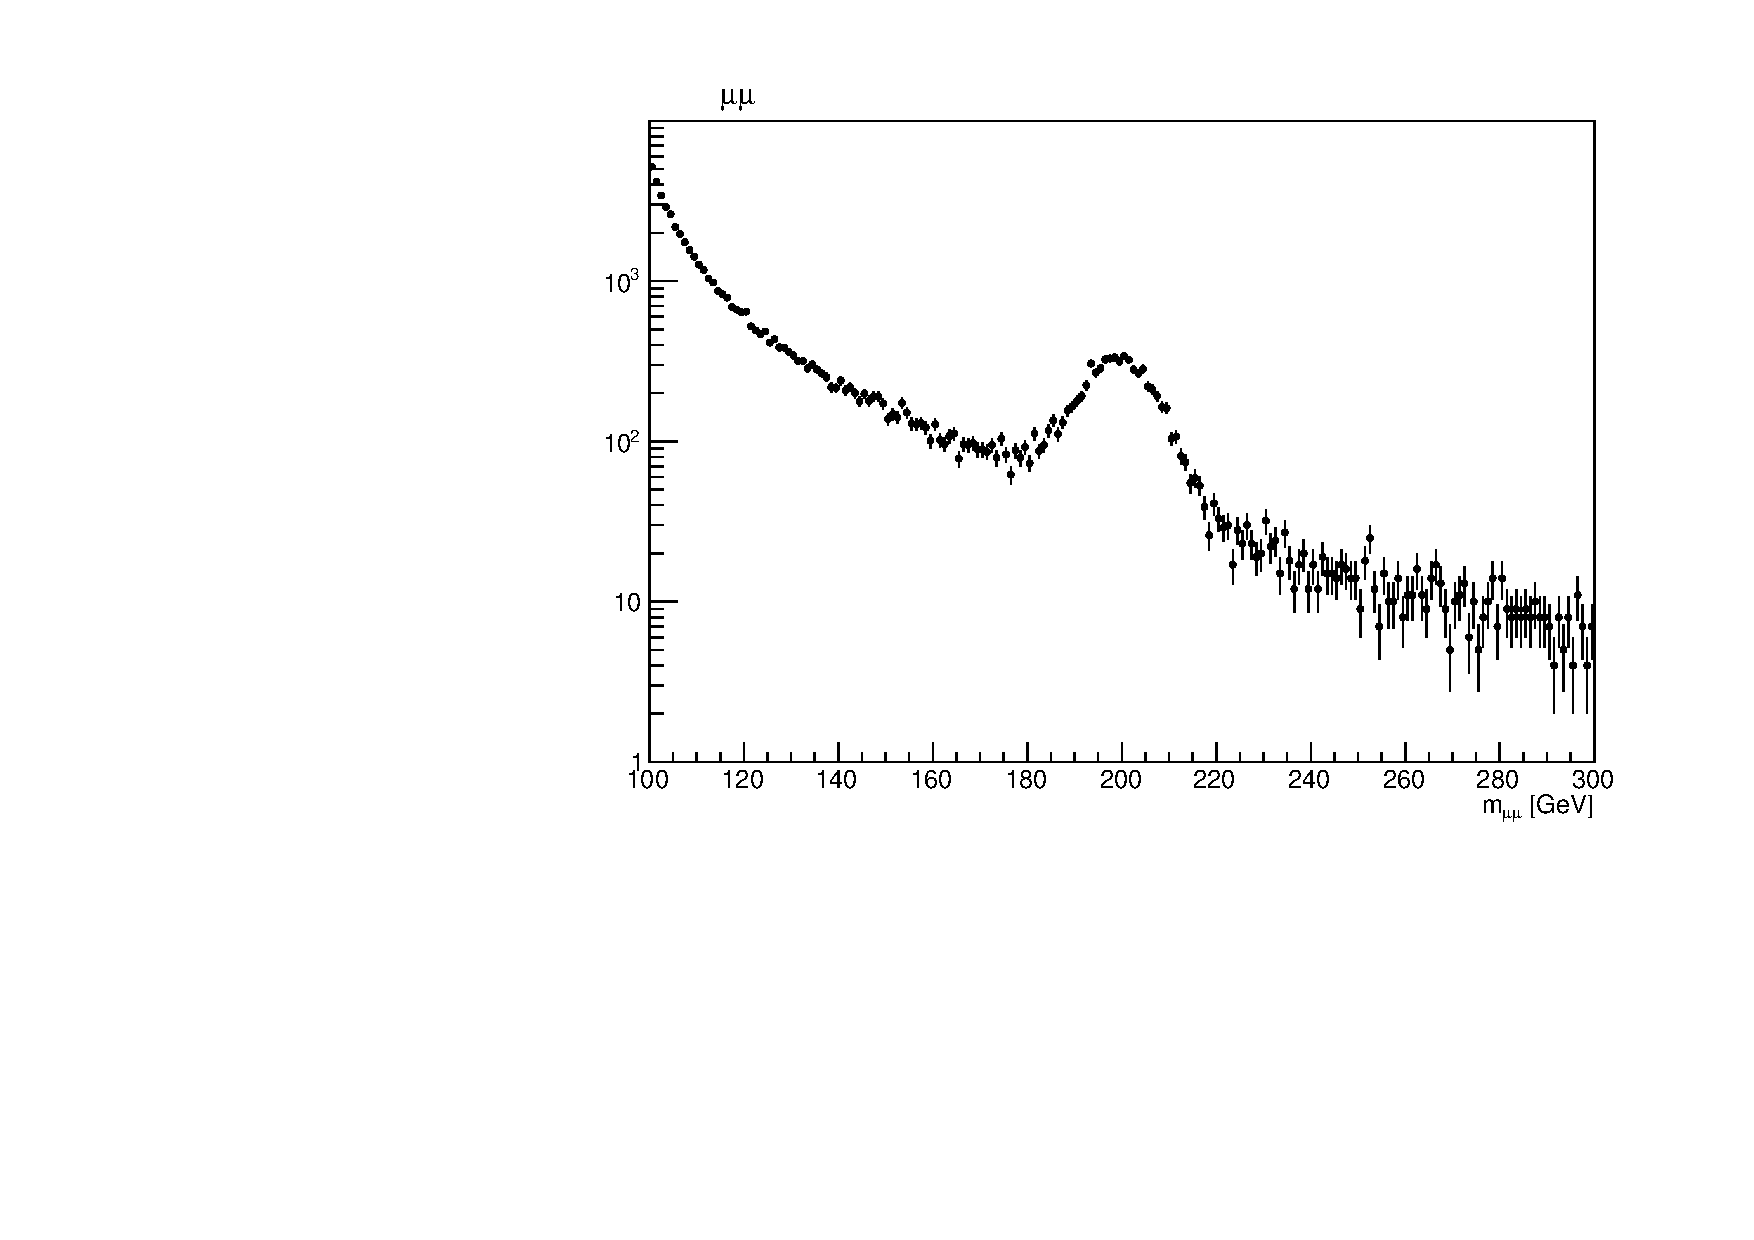
\includegraphics[width=0.5 \textwidth]{/home/kpapad/UG_thesis/Thesis/Analysis/out/Plots/DYJets_test2.pdf}
\caption{The $Y\rightarrow XX$ invariant mass spectrum}
\label{fig:diX}
\end{figure}

\subsection{Energy scale uncertainties}
\label{sec:orgd3ccc28}
\label{sec:Energy_scale_uncertainties}
Energy scale uncertainties have an effect on the transverse momenta \(P_t\) of the produced \(XX\) pair. Such uncertainties are modeled as random noise (Gaussian smearing) to the signal component. To smear the data by \(x\%\), we iterate over every signal event and multiply the transverse momenta by numbers sampled from a Gaussian distribution of \(\mu = 1\) and \(\sigma = x/100\), where \(x\) is the percentage of smearing (each \(P_t\) is multiplied by a different number).

In the present study, we compare the performance of a Boosted Decision Tree (BDT)-based analysis and a fit-based analysis on a given dataset, for various cases of smearing (various values of \(\sigma\)). Table \ref{table:Smearings} summarizes the smearing percentages used for this analysis. The values are chosen such that we examine both cases of mild noise (\(0-5\%\)) up to extreme noise (\(50\%\)). Nevertheless, it should be noted that what is considered as an extreme case or a mild case of smearing is not defined in an absolute manner but rather is related to the mass range of the data upon which the blur is applied.

\begin{table}[h!]
\centering
\begin{tabular}{ |c|  }
 \hline
Percentage of smearing \\
 \hline
$0\%$\\
$5\%$\\
$10\%$\\
$15\%$\\
$20\%$\\
$30\%$\\
$40\%$\\
$50\%$\\
\hline
\end{tabular}
\caption{Summary of the smearing cases that will be studied in this work }
\label{table:Smearings}
\end{table}

\subsection{Analysis Method I: Training a BDT Classifier}
\label{sec:org2ab78e2}
\label{sec:Analysis_method1}
\subsubsection{The Train/Test/Application data sets}
\label{sec:orgc1060da}
\label{sec:Train_test_application_sets}
For the BDT training (and due to the lack of an infinite number of events), the original dataset had to be split into three parts. The training set is used to train the classifier. As the reader may have noticed, the signal events in the original dataset are much less than the background events. This class imbalance makes the training of the model much harder, and for that reason, the training set has been enriched with more (unseen) signal events, so that the two classes have the same number of events. The testing set is used to evaluate the training. For that purpose, the two signal and background classes also have the same number of events. Finally, the application set is used for the analysis. Through trial and error, we noticed that working with smaller statistics enhances the magnitude of statistical fluctuations in the analysis. To avoid such confusion, the application set contains a part of the testing set to ensure large statistics. This doesn't interfere with the training, since the BDT has never seen the testing events during training. Finally, it should be mentioned that in order to have an "apples-to-apples" comparison between the BDT-based analysis and the Fit-based analysis, the application set will be analyzed in both cases. For that reason, the smearing cases that will be discussed for the rest of this chapter will concern only the application set.

Table \ref{table:TrainTestApp} summarizes the number of events used in each dataset.

\begin{table}[h!]
\centering
\begin{tabular}{ |p{3cm}|p{3cm}|p{4cm}|  }
 \hline
Data Set & No.Signal Events & No. Background Events \\
 \hline
Training & 3882 & 3882 \\
Testing & 3881 & 3881 \\
Application & 2973 & 20827 \\
 \hline
\end{tabular}
\caption{Sumarry of the Train Test Application number of events}
\label{table:TrainTestApp}
\end{table}
\subsubsection{Training}
\label{sec:org048945f}
\label{sec:Training}
One of the key aspects of a successful training is the feature space that is being used. Although the Train/Test sets consist of the features described in Table \ref{table:DataSetFeatures}, those features are not optimal for the particular classification problem. The feature space that is found to be optimal for the problem in question consists of five features and is summarized in Table \ref{table:TrainFeatures} and Figure \ref{fig:TrainFeaturesPlot}.

\begin{table}[h!]
\centering
\begin{tabular}{ |p{3.5cm}|p{11cm}| }
 \hline
Feature & Description \\
 \hline
$Pt_{1}$ &  the transverse momentum of the first particle in the XX pair. \\
 \hline
$Pt_{2}$ &the transverse momentum of the second particle in the XX pair. \\
 \hline
$\Delta\phi = \phi_{2} - \phi_{1}$ & the difference in the azimuthal angles between the two particles in the XX pair. \\
 \hline
$\Delta\eta = \eta_{2} - \eta_{1}$ & the difference in the pseudorapidity values between the two particles in the XX pair. \\
 \hline
$\Delta R = \sqrt{\Delta\eta^{2} + \Delta\phi^{2}}$ & the separation in the eta-phi plane between the two particles in the XX pair. \\
 \hline
\end{tabular}
\caption{Sumarry of the features used for training }
\label{table:TrainFeatures}
\end{table}

\begin{figure}[h!]
\centering
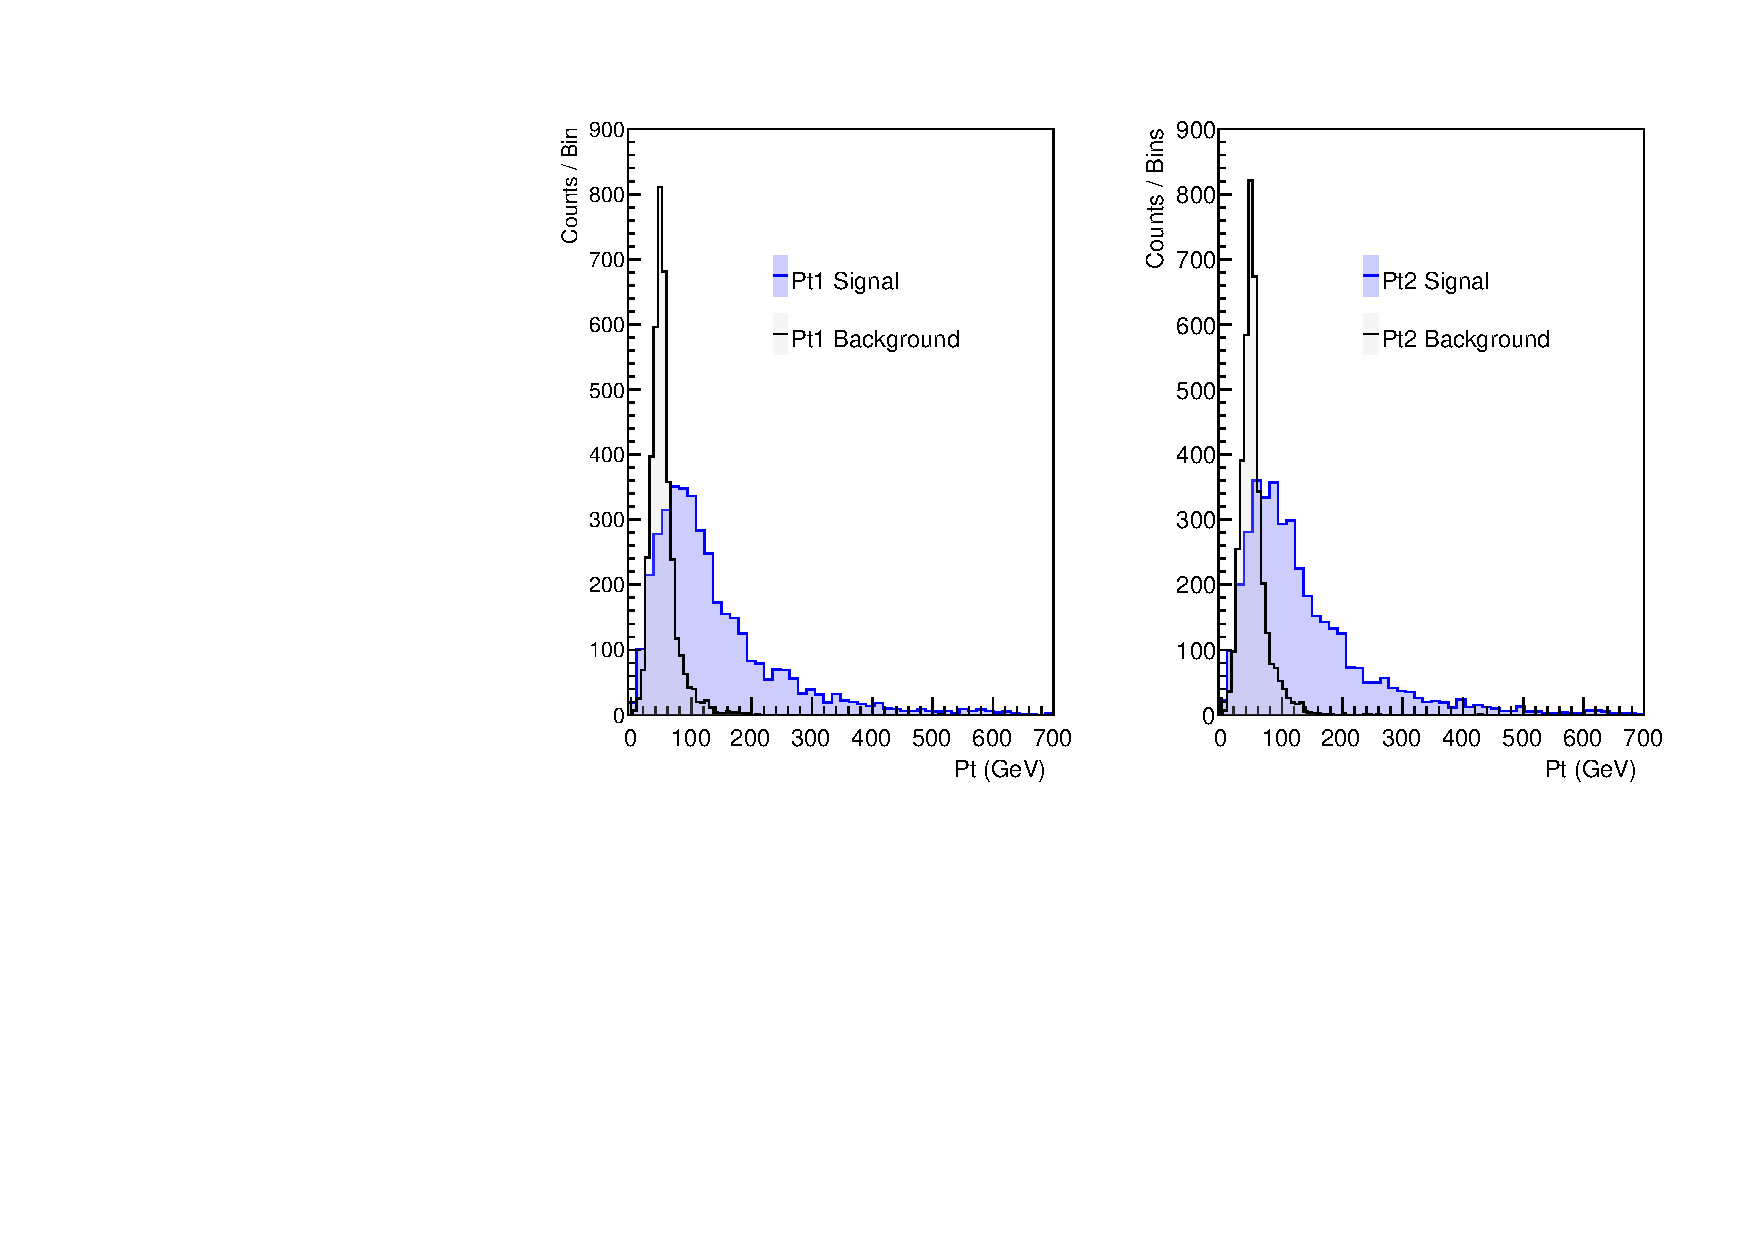
\includegraphics[page=1,width=0.6\textwidth]{/home/kpapad/UG_thesis/Thesis/Analysis/out/Plots/WPhiJets_M200M100300Deltas_varsplot.pdf}
\includegraphics[page=2,width=0.6\textwidth]{/home/kpapad/UG_thesis/Thesis/Analysis/out/Plots/WPhiJets_M200M100300Deltas_varsplot.pdf}
\caption{Sumarry of the features used for training }
\label{fig:TrainFeaturesPlot}
\end{figure}

To assess the performance of the trained model, the Area Under the Receiver Operating Curve (ROC-AUC) is used as a metric. However, it is important to note that in addition to evaluating the model's performance, we also consider the possibility of overfitting. To quantify overfitting, we examine the ratio of the number of training events to the number of testing events at a particular BDT score. If the model is not overtrained, the performance on the training and testing set will be approximately the same, and therefore, the ratio will fluctuate around 1 across the BDT score range.

Figure \ref{fig:BDTplot} displays the BDT score plot of the training and testing set, as well as the corresponding ROC curves. The performance of the model on the testing set yields an AUC score of 0.98. Looking at the Training/Testing ratios, one can notice that they fluctuate around one. The absence of a profound trend in both signal and background ratios implies that the model is not severely overfitted.
\begin{figure}[h]
\centering
\begin{subfigure}{0.49\textwidth}
\centering
\includegraphics[page=5, width=\linewidth]{/home/kpapad/UG_thesis/Thesis/Bdt/out/Plots/WPhiJets_M200M100300DeltasPConf12BDTplot.pdf}
\caption{}
\end{subfigure}
\begin{subfigure}{0.49\textwidth}
\centering
\includegraphics[page=3, width=\linewidth]{/home/kpapad/UG_thesis/Thesis/Bdt/out/Plots/WPhiJets_M200M100300DeltasPConf12BDTplot.pdf}
\caption{}
\end{subfigure}
\caption{A: The BDT score of the Testing and Training sets. B: The roc curves for the training and testing sets}
\label{fig:BDTplot}
\end{figure}
\subsubsection{Application}
\label{sec:org6bb475b}
\label{sec:Application}
The application of the model to the application set is a rather straightforward process. The data are simply "fed" to the model, and the latter performs the classification. The ROC curves for the performance of the trained model on the data for each of the smearing cases of table \ref{table:Smearings} are illustrated in figure \ref{subfig:SmearingROC}.

\begin{figure}[h]
\centering
\begin{subfigure}{0.49\textwidth}
\centering
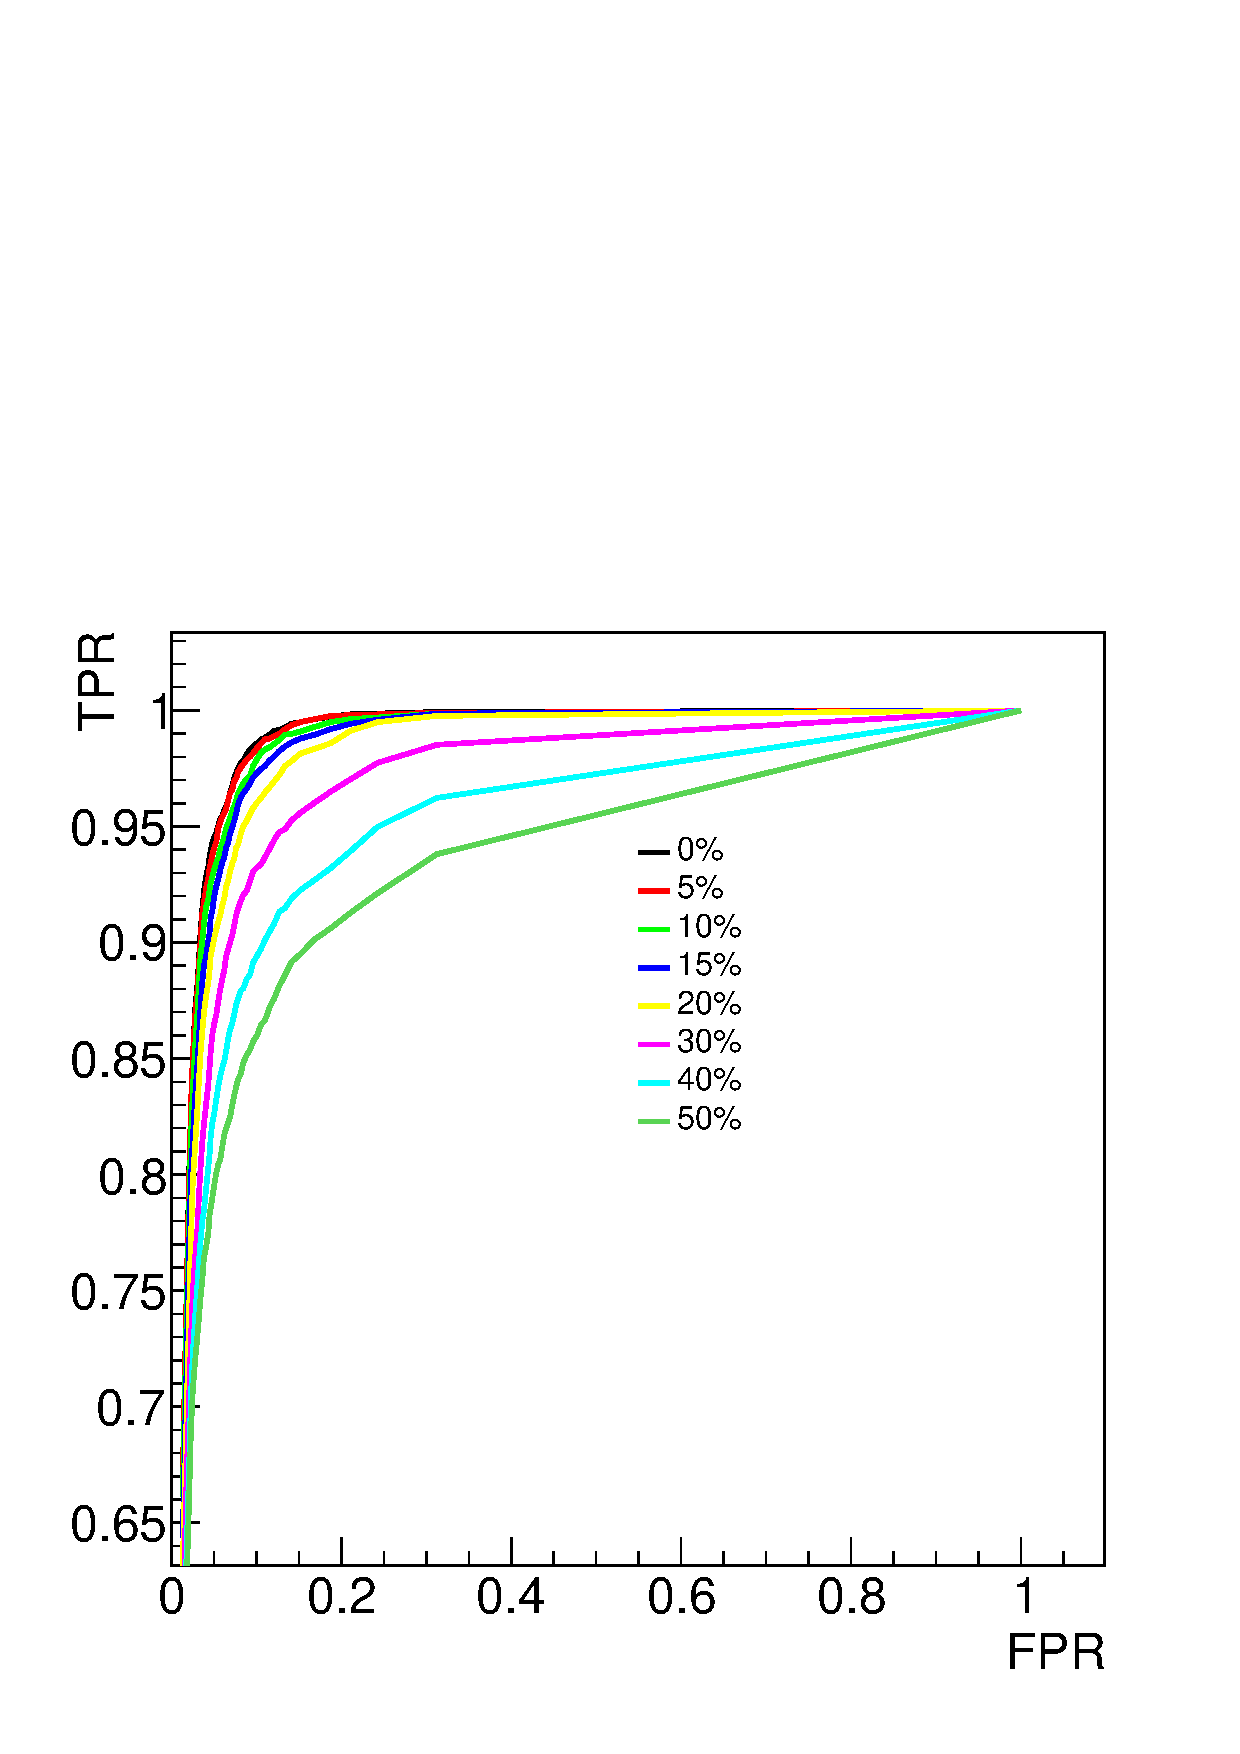
\includegraphics[page=1,width=\linewidth]{/home/kpapad/UG_thesis/Thesis/Bdt/src/WPhiJets_M200M100300_ROCs.pdf}
\caption{}
\label{subfig:SmearingROC}
\end{subfigure}
\begin{subfigure}{0.49\textwidth}
\centering
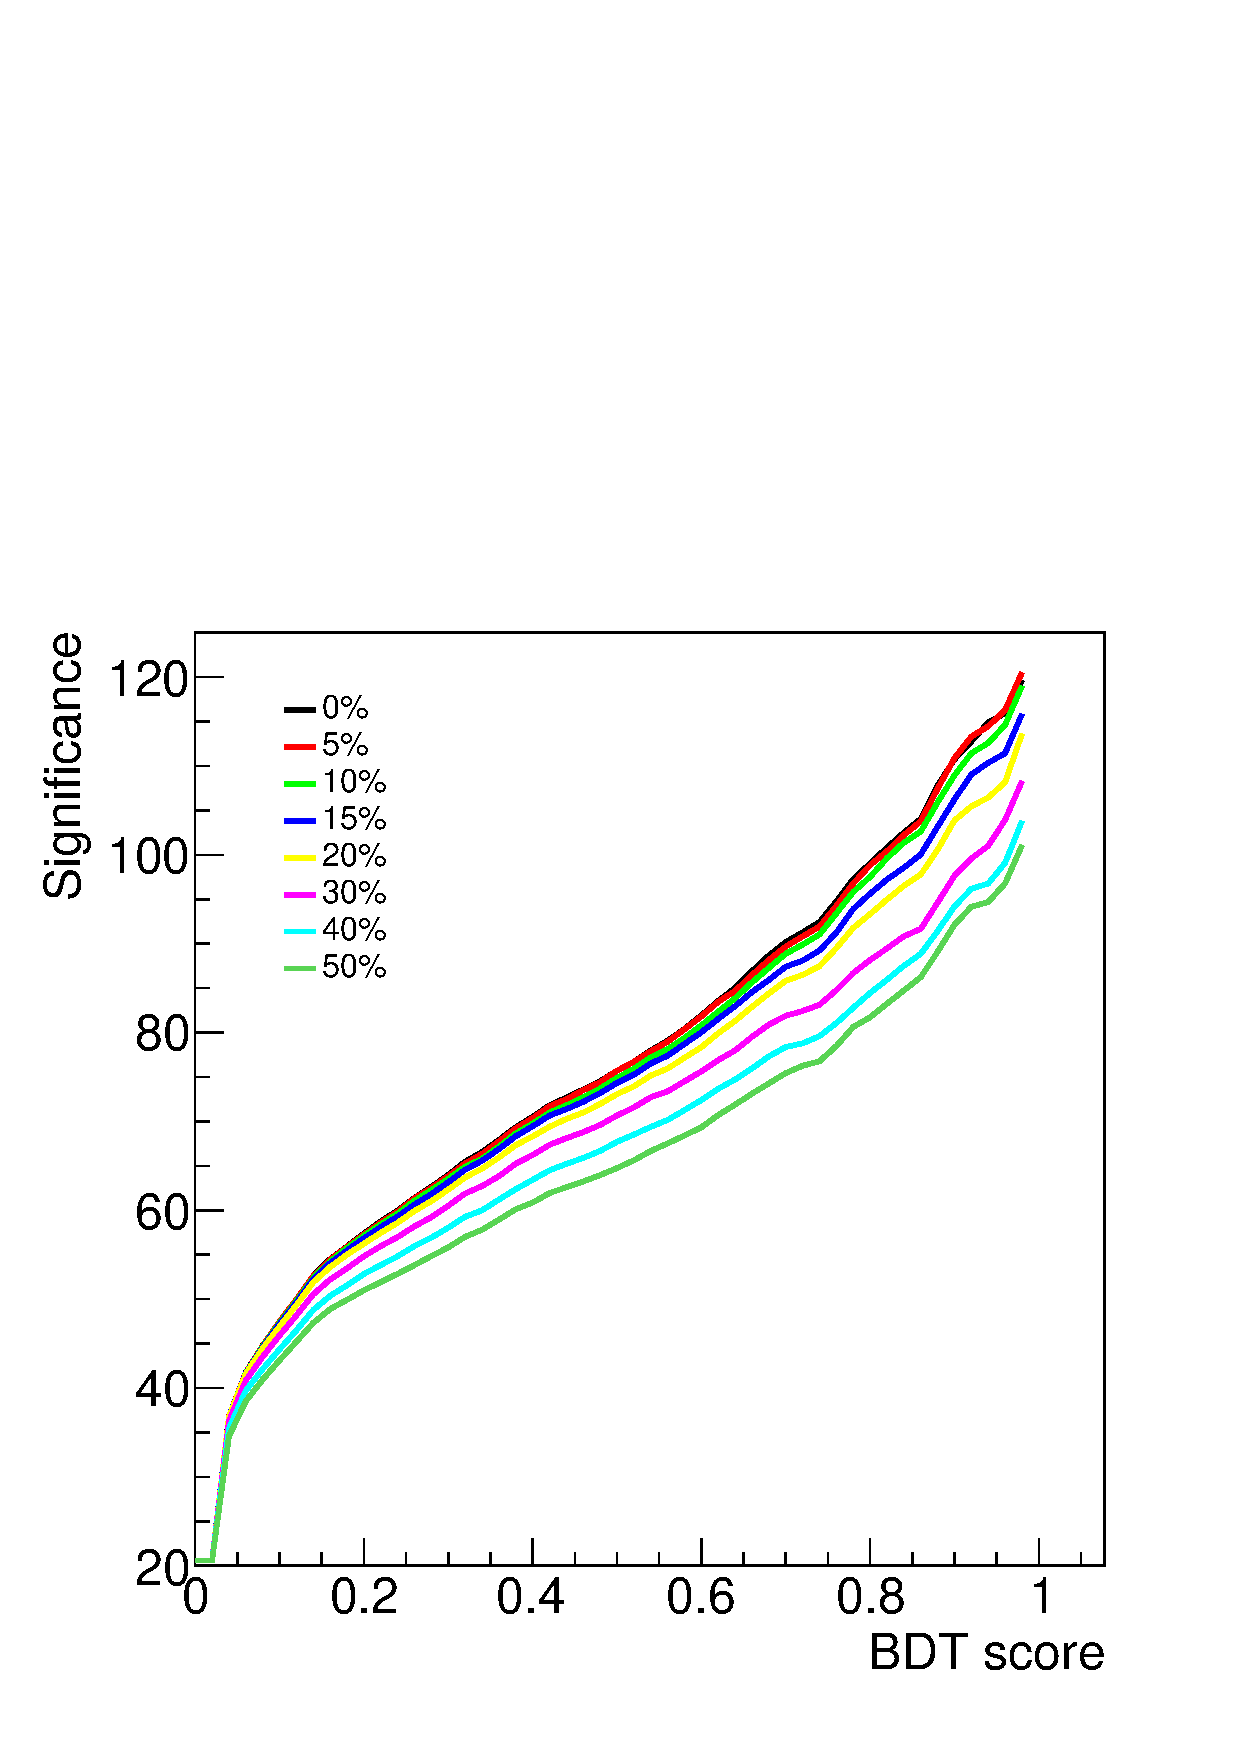
\includegraphics[page=1,width=\linewidth]{/home/kpapad/UG_thesis/Thesis/Bdt/src/WPhiJets_M200M100300_Significance.pdf}
\caption{}
\label{subfig:SigScan}
\end{subfigure}
\caption{a: Summary of the ROC curves for the performance of the model on the data for each smearing case. b: Significances calculated across the BDT score range for the smearing cases of Table \ref{table:Smearings}. The way that these curves are made is analogous to the calculation of the ROC curve.}
\end{figure}

To find the optimal BDT score to place the cut, the whole BDT score range is scanned, and the significance is evaluated in the range [c,1], \(\forall c\in[0,0.98]\) with step size 0.02, same as the bin width of the BDT score histogram(it is pointless to calculate the significance at a single point since it will be 0). The scan of significance for every case of smearing is illustrated in figure \ref{subfig:SigScan}.

Looking at the plot, the cut that gives the best significance is c = 0.98 (the region will be [0.98,1]). Moreover, it is of interest to consider a wider region as well, for the reason that more signal is accepted despite the rejection of less background. To make this argument a bit clearer, let us consider figure \ref{fig:BDTplot}a. At BDT score \textasciitilde{} 7 and onwards, the amount of background events in each bin remains somewhat constant (within statistical fluctuations) while the signal events increase rapidly. It is therefore interesting for our analysis to see how this behavior reflects on the evolution of significance for the various cases of smearing. Looking at figure \ref{subfig:SigScan} again, we conclude that a cut at c = 0.86 is good enough for our purpose.

The results can be seen in Figure \ref{fig:SigEvolBDT} which compares the evolution, in terms of smearing percentage, of the significance for the cuts c = 0.98 and c = 0.86. Table \ref{table:SigBkgBDT} presents the amount of signal and background events present for the two cuts.

\begin{figure}[h]
\centering
\includegraphics[page=2,width=0.5\textwidth]{/home/kpapad/UG_thesis/Thesis/Bdt/src/WPhiJets_M200M100300_Significance.pdf}
\caption{Evolution of significance for the smearing cases of table \ref{table:Smearings}. }
\label{fig:SigEvolBDT}
\end{figure}


\begin{table}[ht]
\centering
\begin{tabular}{|p{2cm}|p{3cm}|p{3cm}|p{3cm}|p{3cm}|}
 \hline
Smearing \%  & No. Sig. Events at BDT cut = 0.86 & No. Bkg.Events at BDT cut = 0.86 & No. Sig. Events at BDT cut = 0.98 & No. Bkg.Events at BDT cut = 0.98  \\
\hline
0 & 2622.0 & 635.0 & 1977.0 & 273.0 \\
5 & 2615.0 & 635.0 & 1991.0  & 273.0 \\
10 & 2586.0 & 635.0 & 1966.0 & 273.0 \\
15 & 2521.0 & 635.0 & 1914.0 & 273.0 \\
20 & 2464.0 & 635.0 & 1877.0 & 273.0 \\
30 & 2310.0 & 635.0 & 1789.0 & 273.0 \\
40 & 2239.0 & 635.0 & 1715.0 & 273.0 \\
50 & 2173.0 & 635.0 & 1670.0 & 273.0 \\
 \hline
\end{tabular}
\caption{Signal and background events at BDT cut 0.86 and 0.98 for different smearing percentages.}
\label{table:SigBkgBDT}
\end{table}
\subsection{Analysis Method II: Fit based analysis}
\label{sec:orgede04ef}
\label{sec:Analysis_method2}
\subsubsection{Invariant mass reconstruction}
\label{sec:org34759a0}
\label{sec:Invariant_mass_reconstruction}
The invariant mass of the XX pair is calculated using the features in Table \ref{table:DataSetFeatures}. The resulting spectrum is shown in Figure \ref{fig:AppMass}.

\begin{figure}[h!]
\centering
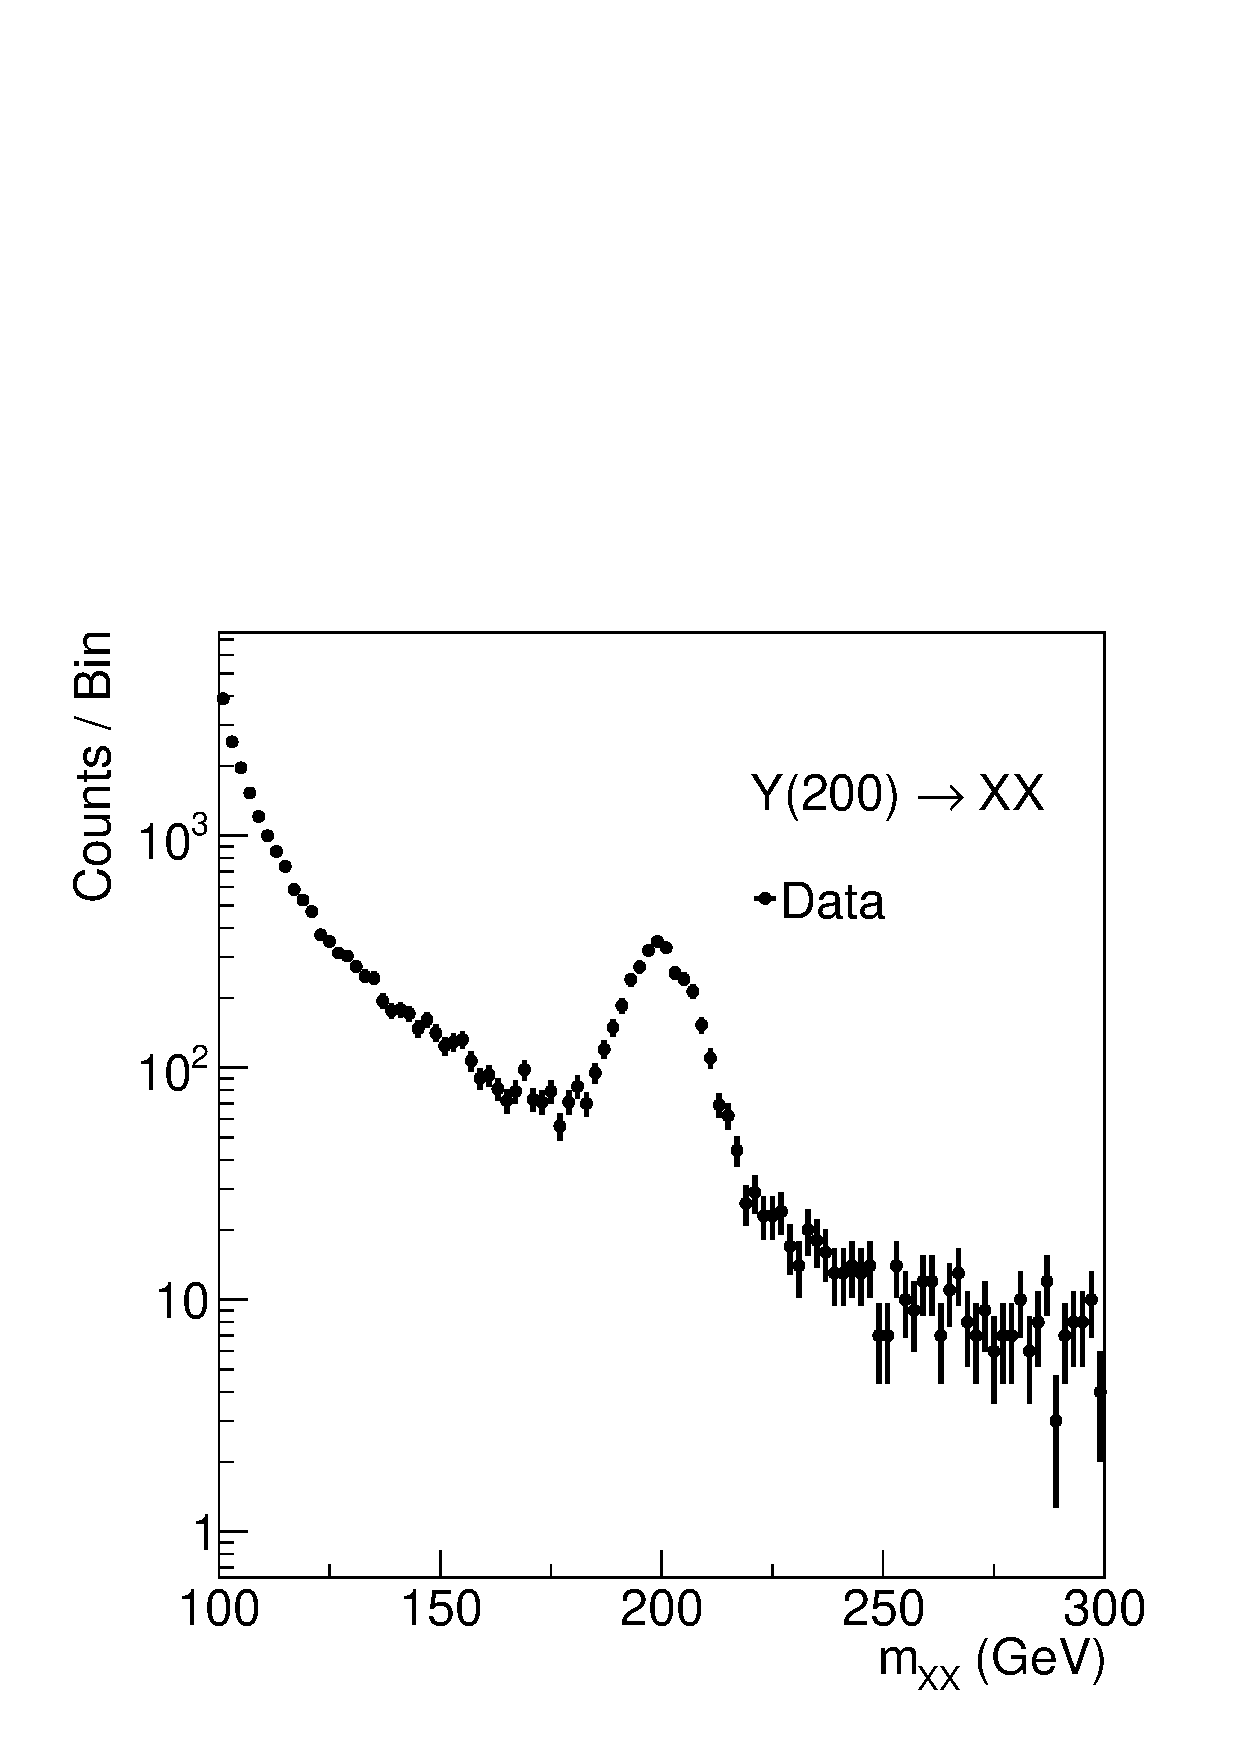
\includegraphics[page=1,width=0.5\textwidth]{/home/kpapad/UG_thesis/Thesis/Analysis/out/Plots/WPhiJets_M200M100300_Application_MassSpectrum.pdf}
\caption{The invariant mass spectrum of the application set}
\label{fig:AppMass}
\end{figure}

Events with invariant mass \(m_{XX} < 120\text{GeV}\) make the background fit significantly harder without contributing significantly to the analysis. Therefore, such events are excluded from this study, and the working mass spectrum is limited to the range \([120, 300]\text{GeV}\).
\subsubsection{Background Fitting}
\label{sec:org6311103}
\label{sec:Background_fitting}
As discussed in previous sections, the applied smearing only affects the signal component of the application set. For this reason, and to simplify the analysis, the background shape is fitted separately and kept constant throughout the signal fits.

Despite this simplification, determining the shape of the background was not a trivial process. Through trial and error, the function shown in Equation \ref{eq:bkgFitFunc} was found to be the best fit.
\begin{equation}
bkg(x) = \alpha + \beta x^{-1/2} + \gamma x^{-1} + \delta x^{3/2}
\label{eq:bkgFitFunc}
\end{equation}
The parameters \(\alpha\), \(\beta\), \(\gamma\), and \(\delta\) are free parameters of the fit. The modeled background is illustrated in Figure \ref{fig:BKGfit}.

\begin{figure}[h!]
\centering
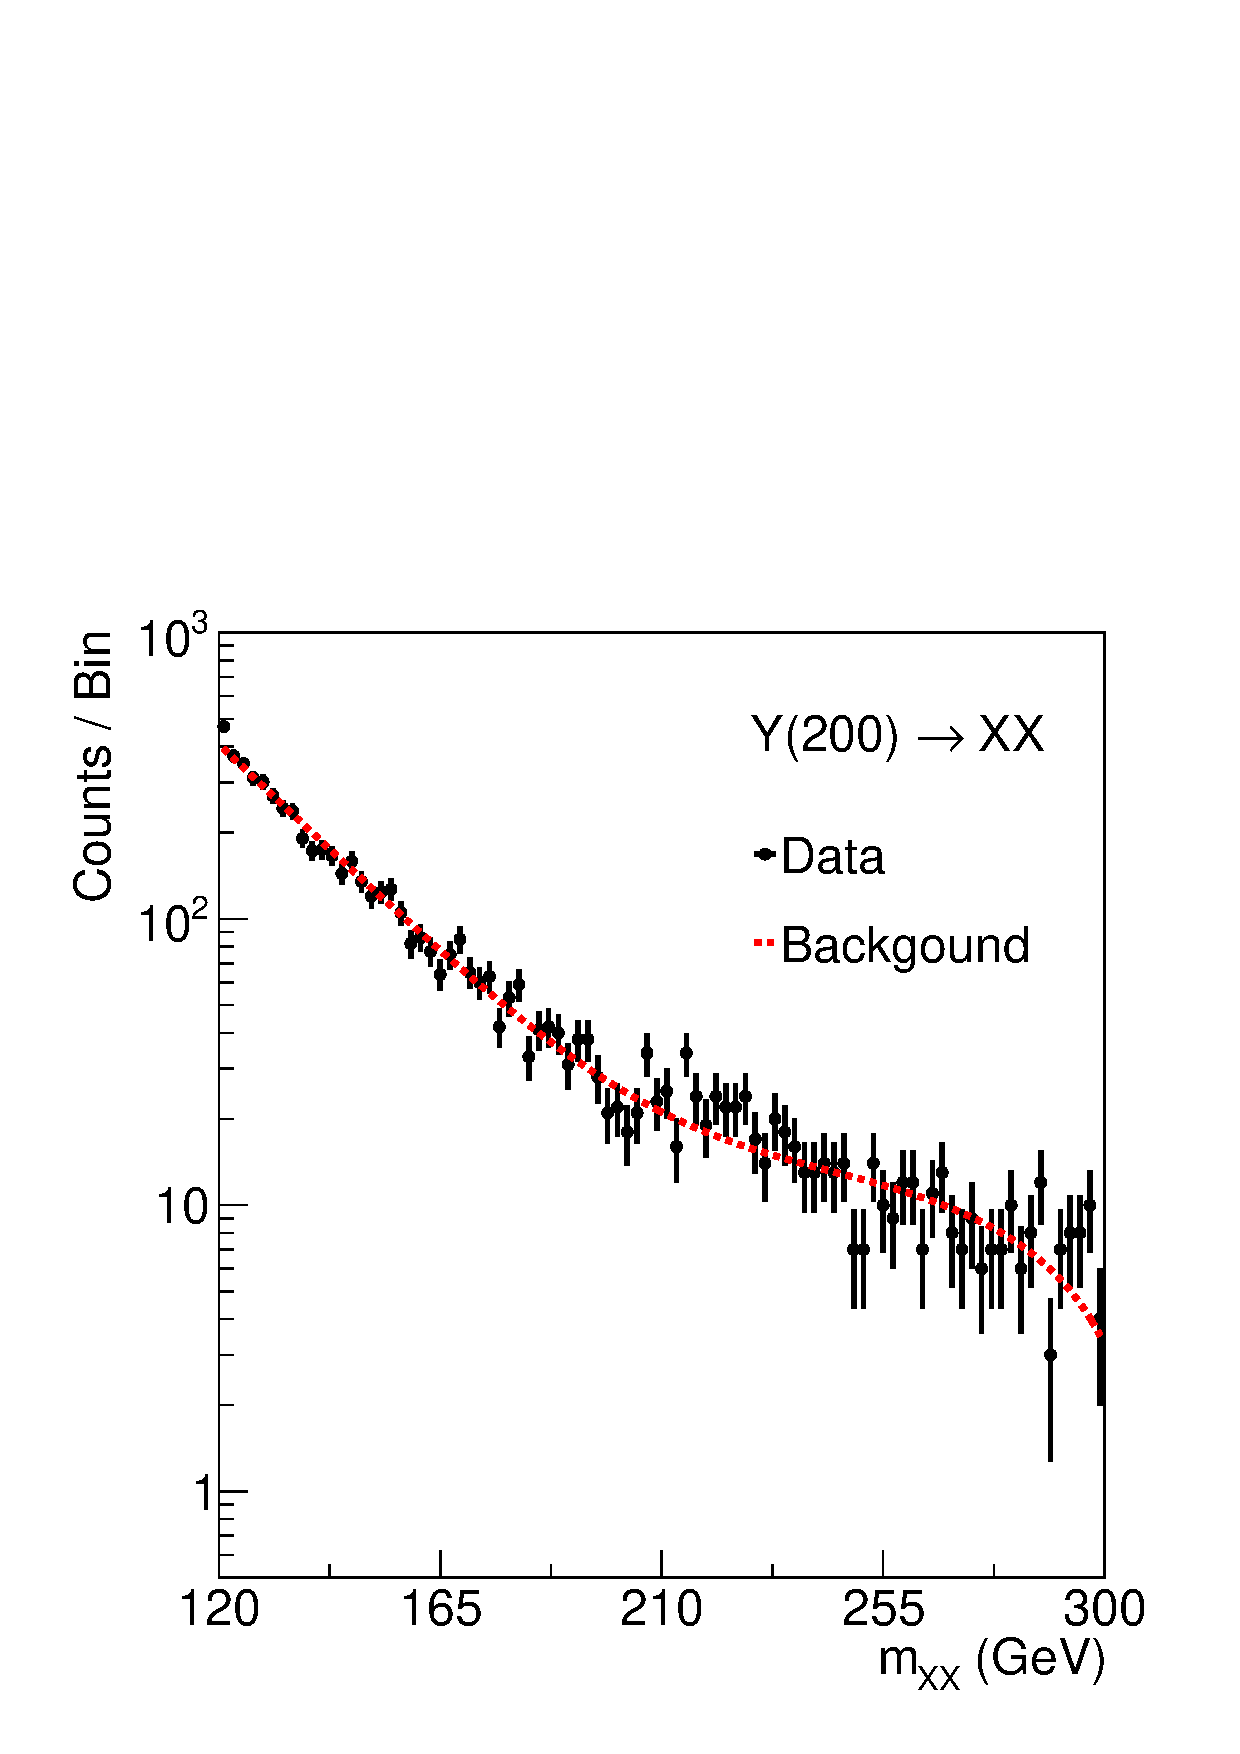
\includegraphics[page=1,width=0.5\textwidth]{/home/kpapad/UG_thesis/Thesis/Analysis/out/Plots/WPhiJets_M200M100300_Application_bkgFit.pdf}
\caption{The fitted background}
\label{fig:BKGfit}
\end{figure}
\subsubsection{Signal Fitting}
\label{sec:org4990f4d}
\label{sec:Signal_fitting}
The signal is fitted using a Gaussian function with \(\sigma\) and magnitude as free parameters, and \(\mu = 200\text{GeV}\) (the mass of the resonance). Figure \ref{fig:fits} shows the fitted invariant mass spectra for smearing percentages of \(0\%\), \(5\%\), \(10\%\), \(15\%\), and \(20\%\). As illustrated in Figure \ref{fig:extremeSmearings}, the signal mass in the extreme cases of \(30\%\text{, }40\%\) and \(50\%\) smearing is indistinguishable from the background. Therefore, attempting to fit those spectra would be a pointless exercise.
\subsubsection{Signal from background separation}
\label{sec:orgcc87bed}
\label{sec:Signal_from_background_separation}
As with the BDT method, we want the region of interest that yields the best significance. To do so, we scan various mass windows around the center of the signal. We scanned six different regions (in the \(0\%\) case), beginning from \(\pm 0.5\sigma\) up to \(\pm 3\sigma\) with a step of \(0.5\sigma\). The results can be seen in Figure \ref{fig:Scan0}. It is evident that the region \(\pm 1.5\sigma\) provides the best performance in terms of significance.
\begin{figure}[h!]
\centering
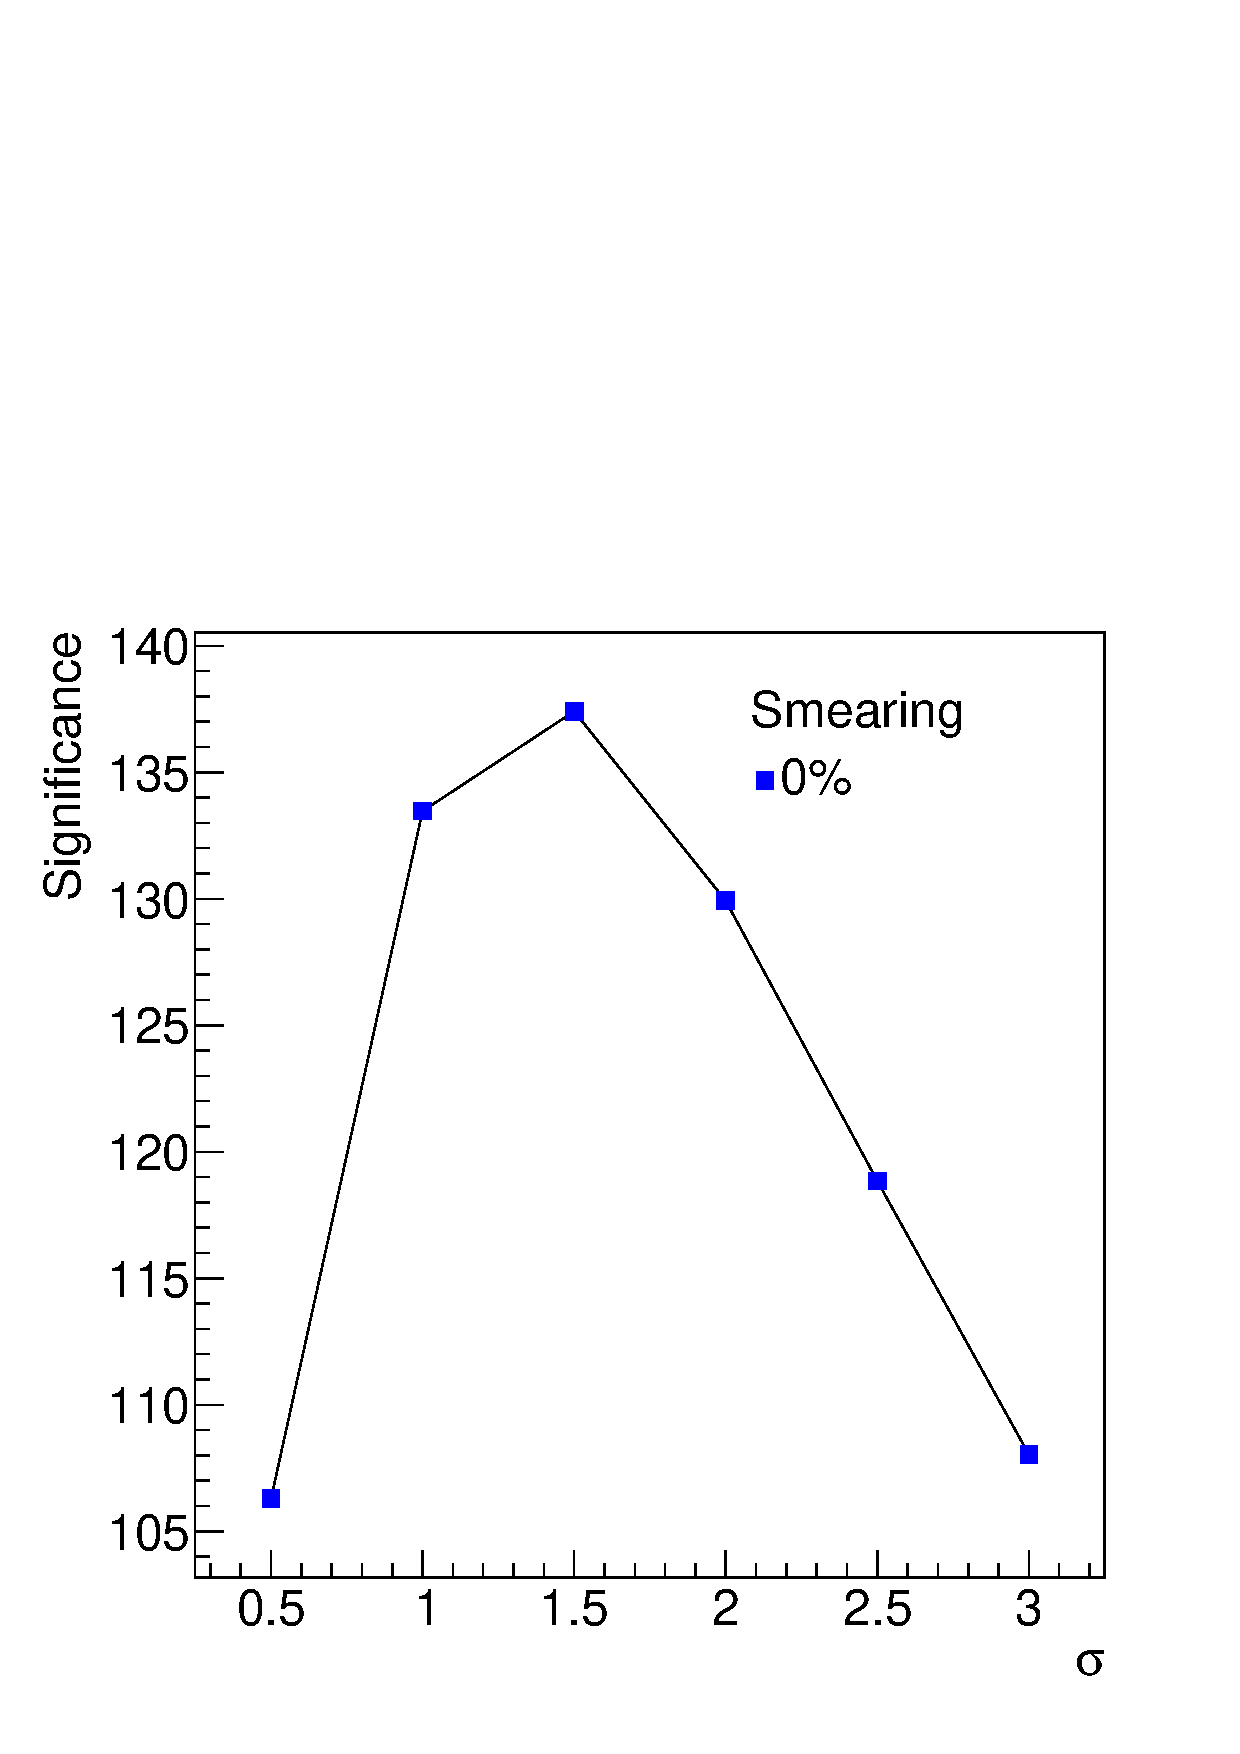
\includegraphics[page=1,width=0.5\textwidth]{/home/kpapad/UG_thesis/Thesis/Analysis/src/WPhiJets_M200M100300_Significance0.pdf}
\caption{Scan of significance for various values of $\sigma$, in the $0\%$ smearing case. We see that the regrion $\pm 1.5\sigma$ around $\mu=200GeV$, gives the best significance.}
\label{fig:Scan0}
\end{figure}

We can then study how the significance changes in the selected region for the various smearing cases in two ways, based on the interpretation of the \(\pm 1.5\sigma\) region. One can interpret \(\sigma\) as the Gaussian spread of the \(0\%\) case and calculate every significance value in the same mass window, resulting in a fixed window study. On the other hand, one can interpret \(\sigma\) as the Gaussian spread of each smearing case. That is, the significance will still be calculated at a \(\pm 1.5\sigma\), but the range will be different based on the different values of \(\sigma\) for every fit, resulting in an adaptive window study. For completeness, we did both studies, and the results are presented in Figure \ref{fig:AdaFixedSig}. Table \ref{table:AdaSigmas}, summarizes the the values of \(\sigma\) (resulting from the fits), and the corresponding mass window for the adaptive widnow search, while table \ref{table:NumSigBkg}, summarizes the amount of signal and background events present in the region of interest of both studies(fixed and adaptive window).
\begin{figure}[h!]
\centering
\includegraphics[page=3,width=0.5\textwidth]{/home/kpapad/UG_thesis/Thesis/Bdt/src/WPhiJets_M200M100300_Significance.pdf}
\caption{Copmarison of the significance evolution as caclulated in the fixed widow and adaptive window case.} 
\label{fig:AdaFixedSig}
\end{figure}
\begin{table}[htbp]
\centering
\begin{tabular}{|p{2cm}|p{2cm}|c|}
 \hline
Smearing \%  & $\sigma$ in GeV & Invarian Mass $\pm 1.5\sigma$ window  in GeV \\
\hline
0 & 7.62 & 23.01\\
5 & 11.15 & 33.47 \\ 
10 & 16.33 & 48.98 \\ 
15 & 22.90 & 68.70 \\ 
20 & 28.87 & 86.60 \\ 
 \hline
\end{tabular}
\caption{Summary of the invariant mass windows used used in adapitve window study. Note that the resulting window of $0\%$ smearing corresponds to the fixed window case as well.}
\label{table:AdaSigmas}
\end{table}
\begin{table}[h!]
\centering
\begin{tabular}{|p{2cm}|p{3cm}|p{3cm}|p{3cm}|p{3cm}|}
 \hline
Smearing \%  & No. Sig. Events (fixed window) & No. Bkg.Events (fixed window) & No. Sig. Events (adaptive window) & No. Bkg.Events (adaptive window)  \\
\hline
0 & 2426 & 311 & 2426 & 311 \\
5 & 2012 & 311 & 2506 & 476 \\
10 & 1511 & 311 & 2539 & 752 \\
15 & 1118 & 311 & 2524 & 1202 \\
20 & 884 & 311 & 2465 & 1662 \\
 \hline
\end{tabular}
\caption{Signal and background events in the 23Gev fixed window region and in the $\pm 1.5\sigma$ adaptive window region, for different smearing percentages.}
\label{table:NumSigBkg}
\end{table}

\subsection{Results}
\label{sec:orgce822e9}
So far, in sections \ref{sec:Analysis_method1} and \ref{sec:Analysis_method2}, we have studied how does a multivariate and a singlevariate calssifcation technique responds to energy scale uncertainties, in a signal from background sepparation task, in the heavy mass region. In this section, we are going to summarize the results and provide commentary regarding each method, in terms of performance and robustness. Moreover will will draw a comparizon between the two methods.

\begin{figure}[h!]
\centering
\includegraphics[page=4,width=0.5\textwidth]{/home/kpapad/UG_thesis/Thesis/Bdt/src/WPhiJets_M200M100300_Significance.pdf}
\caption{ Comparison of the perfomance of the BDT and Fit based analysis, in terms of sifnificance,  as a function of the smearing cases. We can see that BDT based analysis, is more robust.}
\label{fig:BdtFitSig}
\end{figure}

Figure \ref{fig:BdtFitSig}, compares the significance yielded by each method, as a function of smearing. 
Even though, at \(0\%\) of smearing, the fit based method, yields a better significance than the BDT method, the bdt is more robust in general. To explain this, on must pay close attention to the feature space used for the training. The classifier learns not only the energy related Pts of the X particles, but also the geometrical features, \(\Delta\phi\text{, }\Delta R\text{ and }\Delta\eta\). As discribed in section \ref{sec:Energy_scale_uncertainties}, smearing has an effect only on the Pt variables, while the spatial features remain invariant under such process. That is, the BDT model, learns to classify the signal, using features that do not change through out the smearing process, and is therefore able to deliver a better performance, when compared to the fit based analysis, which only makes use of the invariant mass, a feature that gets heavilly altered by uncertainties on the energy scale as figures \ref{fig:fits} and \ref{fig:extremeSmearings} indicate. 

\begin{figure}[hbpt]
\centering
\begin{subfigure}{0.45\textwidth}
\centering
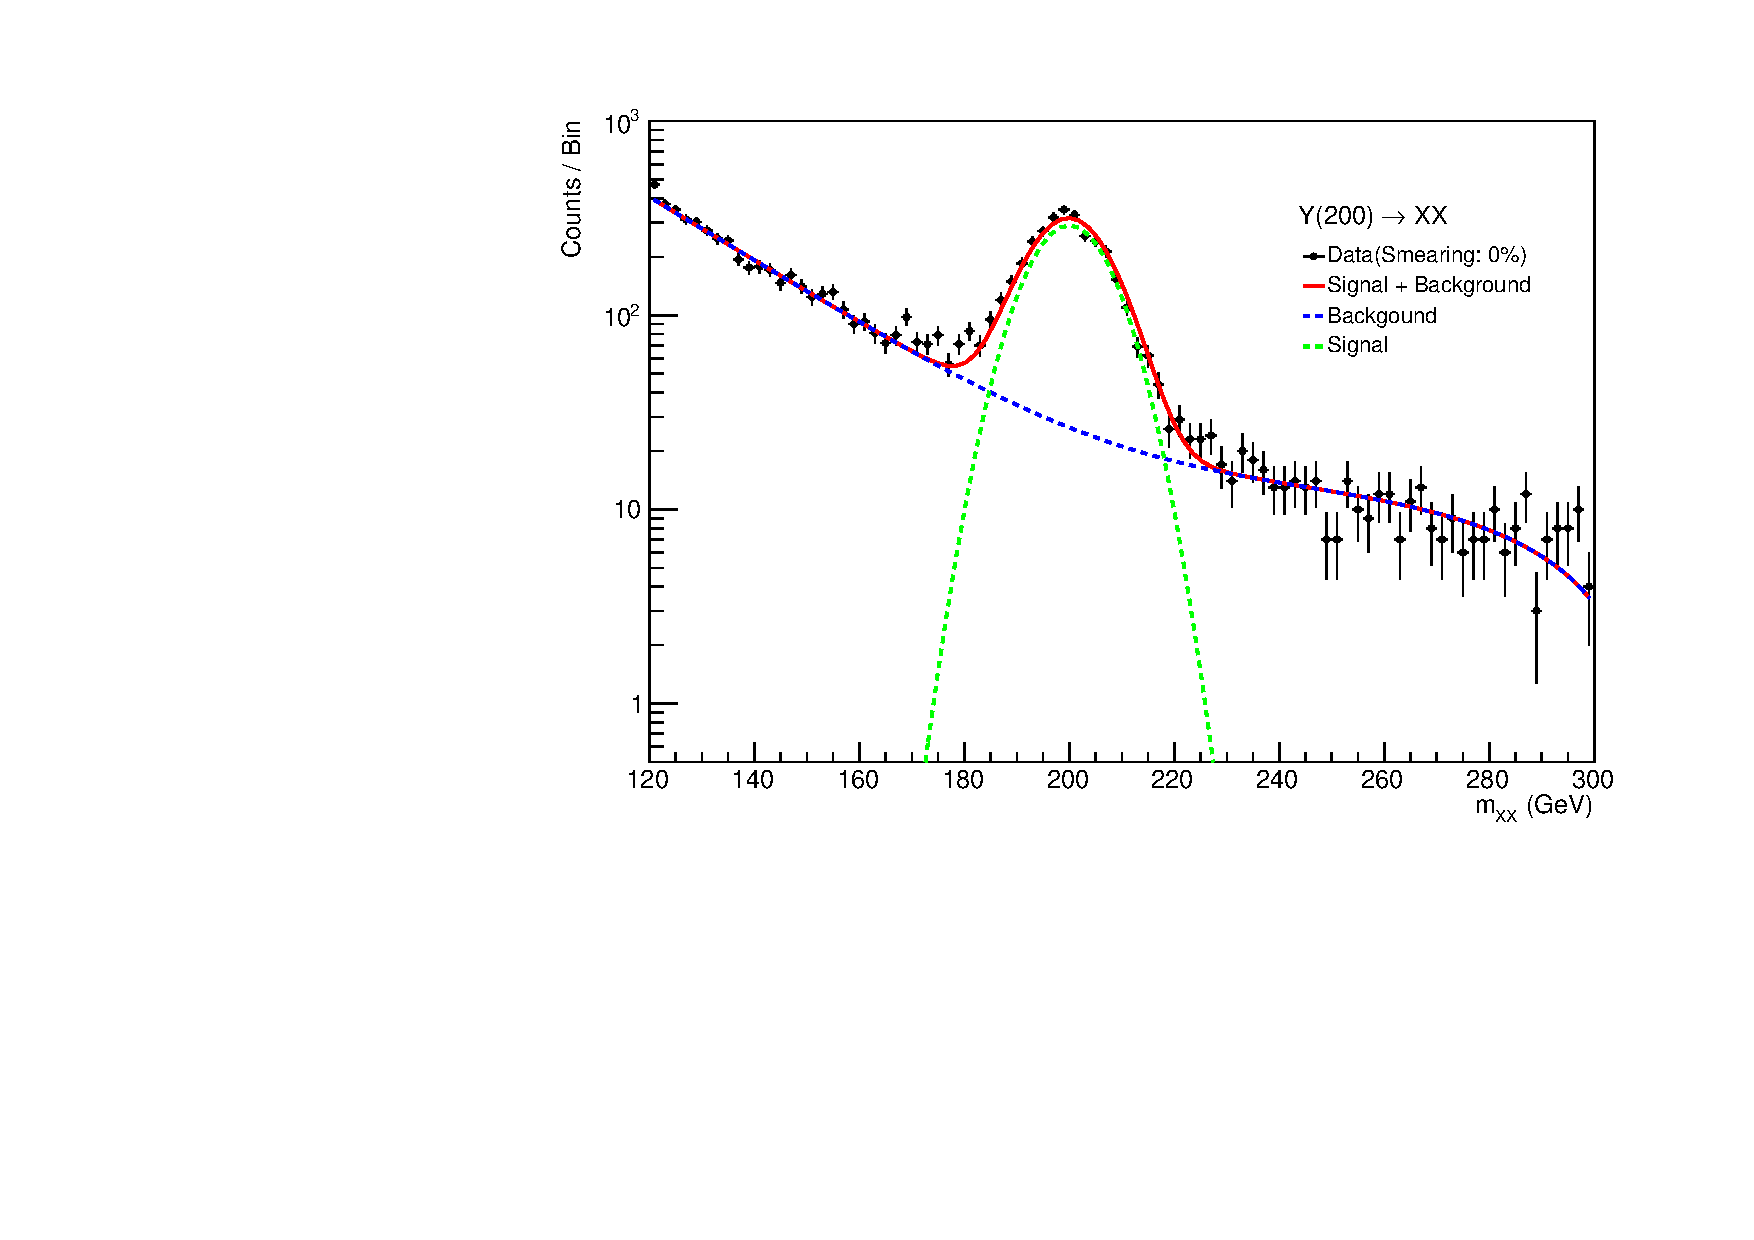
\includegraphics[page=1,width=\linewidth]{/home/kpapad/UG_thesis/Thesis/Analysis/src/WPhiJets_M200M100300_FitALL.pdf}
\caption{}
\end{subfigure}
\begin{subfigure}{0.45\textwidth}
\centering
\includegraphics[page=2,width=\linewidth]{/home/kpapad/UG_thesis/Thesis/Analysis/src/WPhiJets_M200M100300_FitALL.pdf}
\caption{}
\end{subfigure}

\begin{subfigure}{0.45\textwidth}
\centering
\includegraphics[page=3,width=\linewidth]{/home/kpapad/UG_thesis/Thesis/Analysis/src/WPhiJets_M200M100300_FitALL.pdf}
\caption{}
\end{subfigure}
\begin{subfigure}{0.45\textwidth}
\centering
\includegraphics[page=4,width=\linewidth]{/home/kpapad/UG_thesis/Thesis/Analysis/src/WPhiJets_M200M100300_FitALL.pdf}
\caption{}
\end{subfigure}

\begin{subfigure}{0.45\textwidth}
\centering
\includegraphics[page=5,width=\linewidth]{/home/kpapad/UG_thesis/Thesis/Analysis/src/WPhiJets_M200M100300_FitALL.pdf}
\caption{}
\end{subfigure}
\caption{Fits for the following smearing cases a: $0\%$, b:$5\%$, c:$10\%$, d:$15\%$, e:$20\%$}
\label{fig:fits}
\end{figure}

\begin{figure}[hbpt]
\centering
\begin{subfigure}{0.45\textwidth}
\centering
\includegraphics[page=6,width=\linewidth]{/home/kpapad/UG_thesis/Thesis/Analysis/src/WPhiJets_M200M100300_FitALL.pdf}
\caption{}
\end{subfigure}
\begin{subfigure}{0.45\textwidth}
\centering
\includegraphics[page=7,width=\linewidth]{/home/kpapad/UG_thesis/Thesis/Analysis/src/WPhiJets_M200M100300_FitALL.pdf}
\caption{}
\end{subfigure}

\begin{subfigure}{0.45\textwidth}
\centering
\includegraphics[page=8,width=\linewidth]{/home/kpapad/UG_thesis/Thesis/Analysis/src/WPhiJets_M200M100300_FitALL.pdf}
\caption{}
\end{subfigure}
\caption{Invariant mass spectra for the extreme smearing cases of : a:$30\%$, b:$40\%$ and c:$50\%$. The signal seems indistinguishable from the background in these cases, and therefore a fit based saparation cannot work.}
\label{fig:extremeSmearings}
\end{figure}

\newpage
\section{Search for light \(Y \rightarrow XX\)}
\label{sec:org59adc41}
\label{sec:Light_search_Y_to_XX}
\subsection{The light \(Y\rightarrow XX\) channel}
\label{sec:orgabd932d}
\label{Light_y_to_xx}
Similar to the previous study, the dataset used in the present analysis, is composed from a variety of pre-existing Monte Carlo (MC) samples, out of which only generator-level dileptonic final states are selected. The diobject invariant mass is in the range between 50 and 75 GeV, and no further kinematic constraints were placed in the event selection. Finally, the features of the set are summarized in Table \ref{table:DataSetFeatures}, and the invariant mass spectrum of the current decay is illustrated in figure \ref{fig:LightMassSpectrum}. It should be noted that in the study of such a generic process, there is no clear argument regarding a specific signal-to-background number of events ratio. Thus, the number of background and signal events is selected in a somewhat arbitrary manner, with the only condition being the minimization of statistical fluctuations.
\begin{figure}[h]
\centering
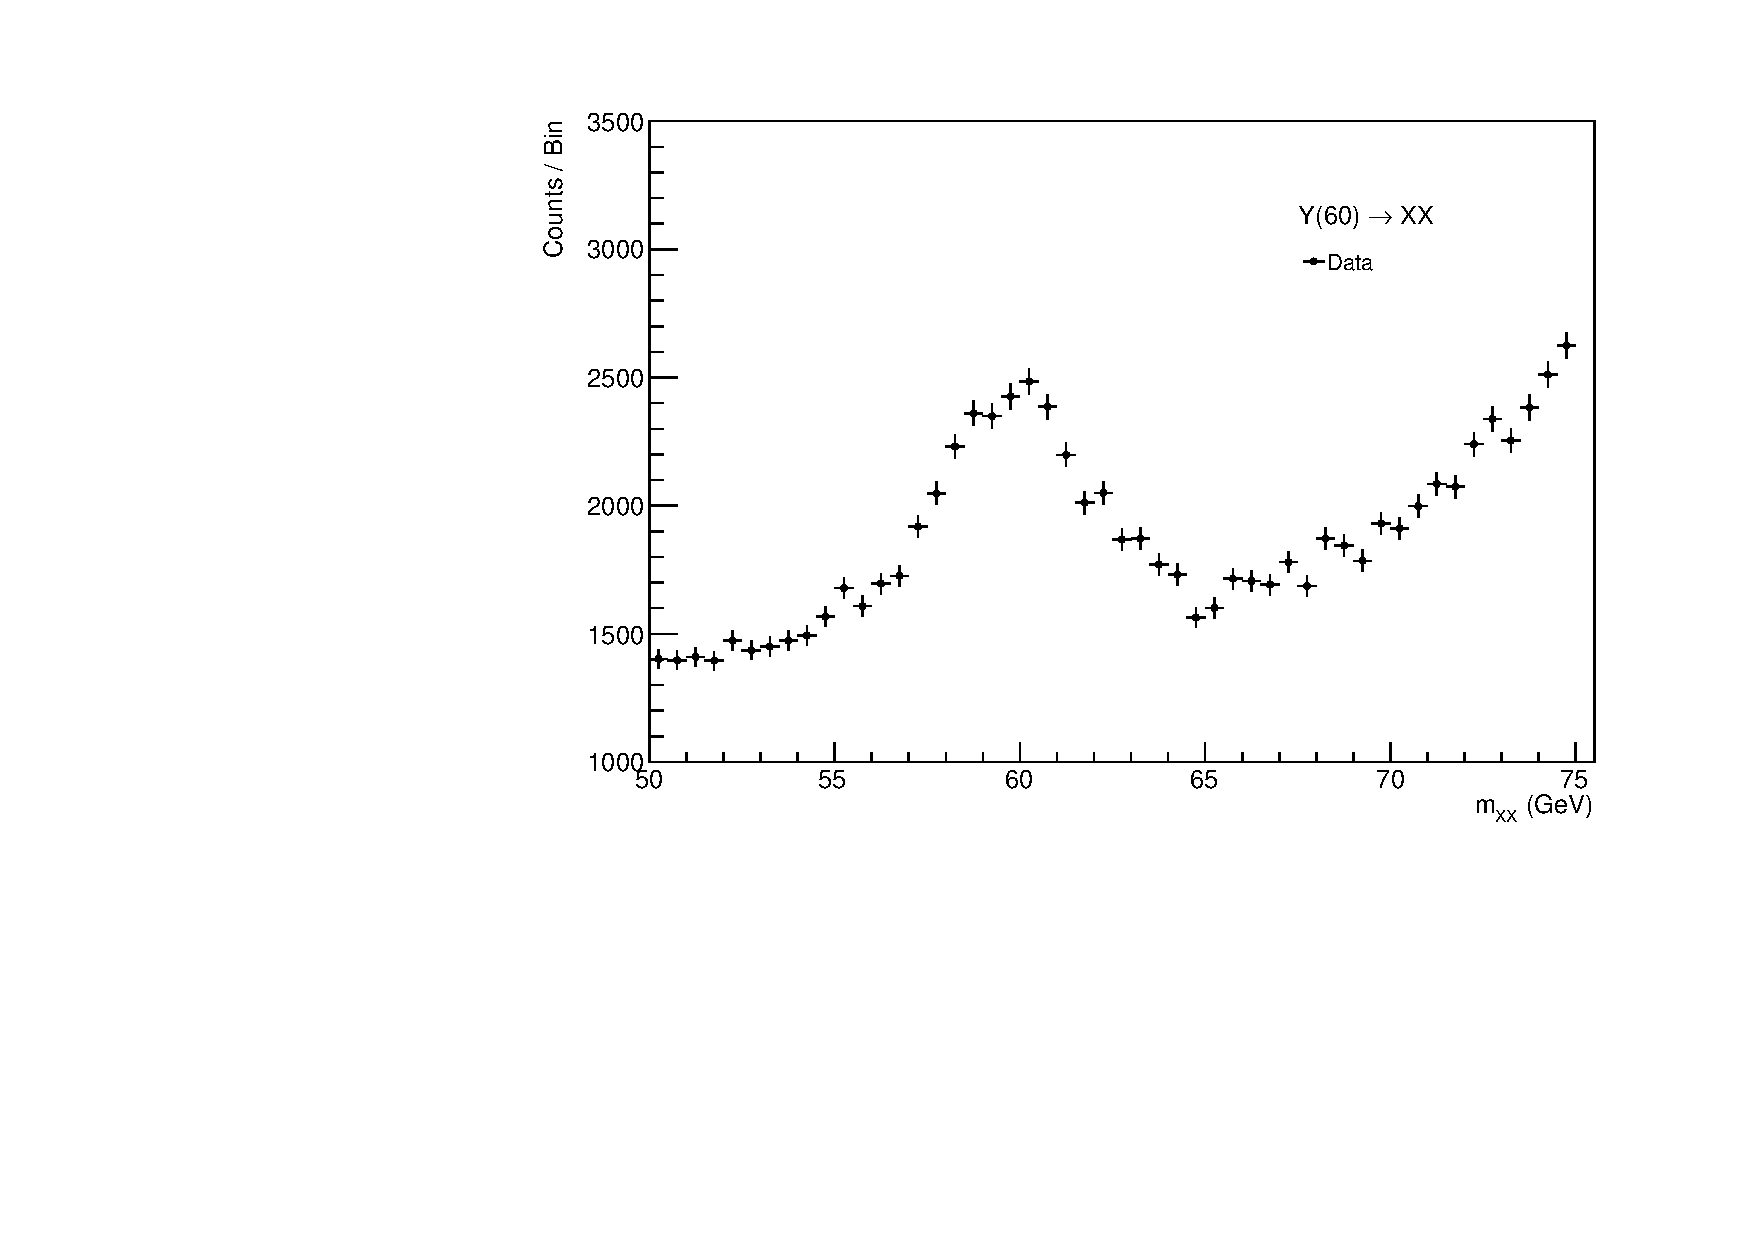
\includegraphics[width=0.5 \textwidth]{/home/kpapad/UG_thesis/Thesis/Analysis/out/Plots/DYJets_M60M5080_MassHist.pdf}
\caption{The $Y\rightarrow XX$ invariant mass spectrum}
\label{fig:LightMassSpectrum}
\end{figure}

\subsection{Energy scale uncertainties}
\label{sec:org56959c3}
\label{sec:Light_energy_scale_uncertainties}
The implementation of energy scale uncertainties in the present dataset is, once again, the same as in the heavy mass study presented in section \ref{sec:Energy_scale_uncertainties}, with the only difference being the percentage of smearing applied. For the particular invariant mass range, the available number of events is significantly lower, and therefore the effect of energy scale uncertainties on the mass is more significant. For that reason, we applied less smearing to the dataset, but nevertheless, we will study cases of mild and extreme smearing. Table \ref{table:LightSmearings} summarizes the cases that will be studied in the following sections.
\begin{table}[h!]
\centering
\begin{tabular}{ |c|  }
 \hline
Percentage of smearing \\
 \hline
$0\%$\\
$5\%$\\
$7\%$\\
$10\%$\\
$12\%$\\
\hline
\end{tabular}
\caption{Summary of the smearing cases that will be studied in the light mass search. }
\label{table:LightSmearings}
\end{table}
\subsection{Analysis method I: Training a BDT Classifier}
\label{sec:org6370180}
\subsubsection{The Train/Test/Application data sets}
\label{sec:orgceb51c1}
\label{sec:Light_train_test_application}
The number of training, testing, and application events is summarized in table \ref{table:LightTrainTestAppEvents}. Comparable to  section \ref{sec:Train_test_application_sets}, a part of the testing events was injected into the application set. However, due to a lack of extra signal, no additional events were used for the Training and Testing set.
\begin{table}[h!]
\centering
\begin{tabular}{ |p{3cm}|p{3cm}|p{4cm}|  }
 \hline
Data Set & No.Signal Events & No. Background Events \\
 \hline
Training & 3638 & 3638 \\
Testing & 3638 & 3638 \\
Application & 3638 & 29077 \\
 \hline
\end{tabular}
\caption{Sumarry of the Train Test Application number of events}
\label{table:LightTrainTestAppEvents}
\end{table}

\subsubsection{Training}
\label{sec:org7ed8c8f}
\label{sec:Light:Training}
The feature space that results in the best model is still that of table \ref{table:TrainFeatures}. An illustration of the current features is shown in figure \ref{fig:LightFeatures}.
\begin{figure}[h]
\centering
\includegraphics[page=1,width=0.6\textwidth]{/home/kpapad/UG_thesis/Thesis/Analysis/out/Plots/WPhiJets_M60M5080DeltasVarsPlots.pdf}
\includegraphics[page=2,width=0.6\textwidth]{/home/kpapad/UG_thesis/Thesis/Analysis/out/Plots/WPhiJets_M60M5080DeltasVarsPlots.pdf}
\caption{Sumarry of the features used for training }
\label{fig:LightFeatures}
\end{figure}

Figure \ref{subfig:LightBdtPlot} illustrates the BDT score of the trained model on the training and testing sets, while the corresponding ROC curves are shown in figure \ref{subfig:LightROCCurves}. The model's performance is assessed using the ROC curve and the AUC score. To evaluate overfitting, the ratio of the number of training events to the number of testing events at a particular BDT score is examined. Looking at figure \ref{subfig:LightBdtPlot}, the ratio of testing and training events fluctuates around one, indicating that the model is not severely overfit. Moreover, the AUC score that this model yields on the training events is 0.90, significantly lower than that of the model that was trained for the classification of the heavy mass dataset.
\begin{figure}[h]
\centering
\begin{subfigure}{0.49\textwidth}
\centering
\includegraphics[page=5, width=\linewidth]{/home/kpapad/UG_thesis/Thesis/Bdt/out/Plots/WPhiJets_M60M5080DeltasPConf13BDTplot.pdf}
\caption{}
\label{subfig:LightBdtPlot}
\end{subfigure}
\begin{subfigure}{0.49\textwidth}
\centering
\includegraphics[page=3, width=\linewidth]{/home/kpapad/UG_thesis/Thesis/Bdt/out/Plots/WPhiJets_M60M5080DeltasPConf12BDTplot.pdf}
\caption{}
\label{subfig:LightROCCurves}
\end{subfigure}
\caption{A: The BDT score of the Testing and Training sets. B: The roc curves for the training and testing sets}
\end{figure}

\subsubsection{Application}
\label{sec:orgebb08bf}
\label{sec:Light_application}
The model's classification performance, on the classification sets, can be assessed by looking at figure \ref{fig:LightROCSIG}, which illustrates the ROC curves and the corresponding significances as a function of the BDT score, for the smearing cases of table \ref{table:LightSmearings}. It is evident that the model is not outstandingly affected by smearing, and thus, there is no point in selecting any other than the BDT score that yields the best significance. That is, placing the cut at BDT score = 0.96. The significance as a function of smearing, for the given cut can be seen in figure \ref{fig:LightSigEvolBDT}. Table \ref{table:LightNumSIGBKG} summarizes the amount of signal and background events present, for the selected cut.
\begin{figure}[h]
\centering
\begin{subfigure}{0.49\textwidth}
\centering
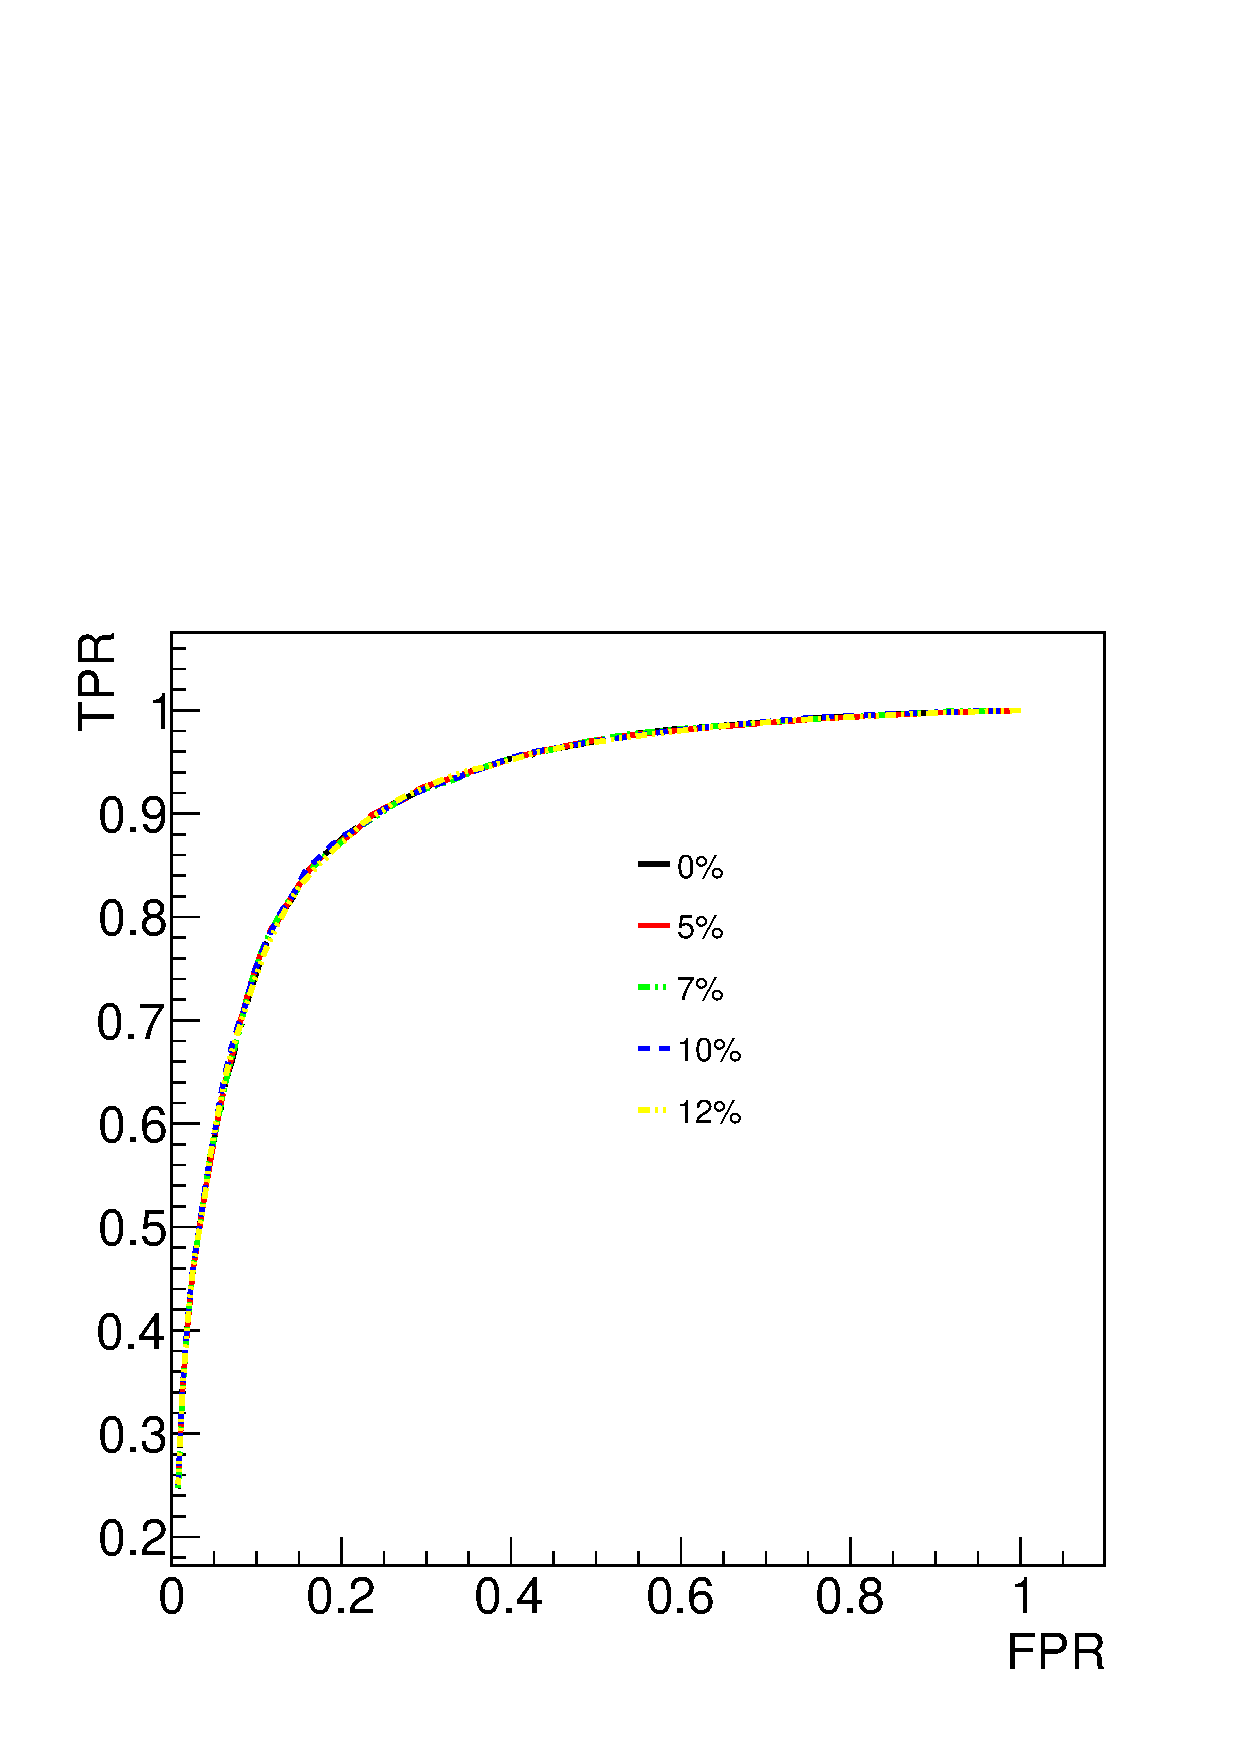
\includegraphics[page=1,width=\linewidth]{/home/kpapad/UG_thesis/Thesis/Bdt/src/WPhiJets_M60M5080_ROCs.pdf}
\caption{}
\end{subfigure}
\begin{subfigure}{0.49\textwidth}
\centering
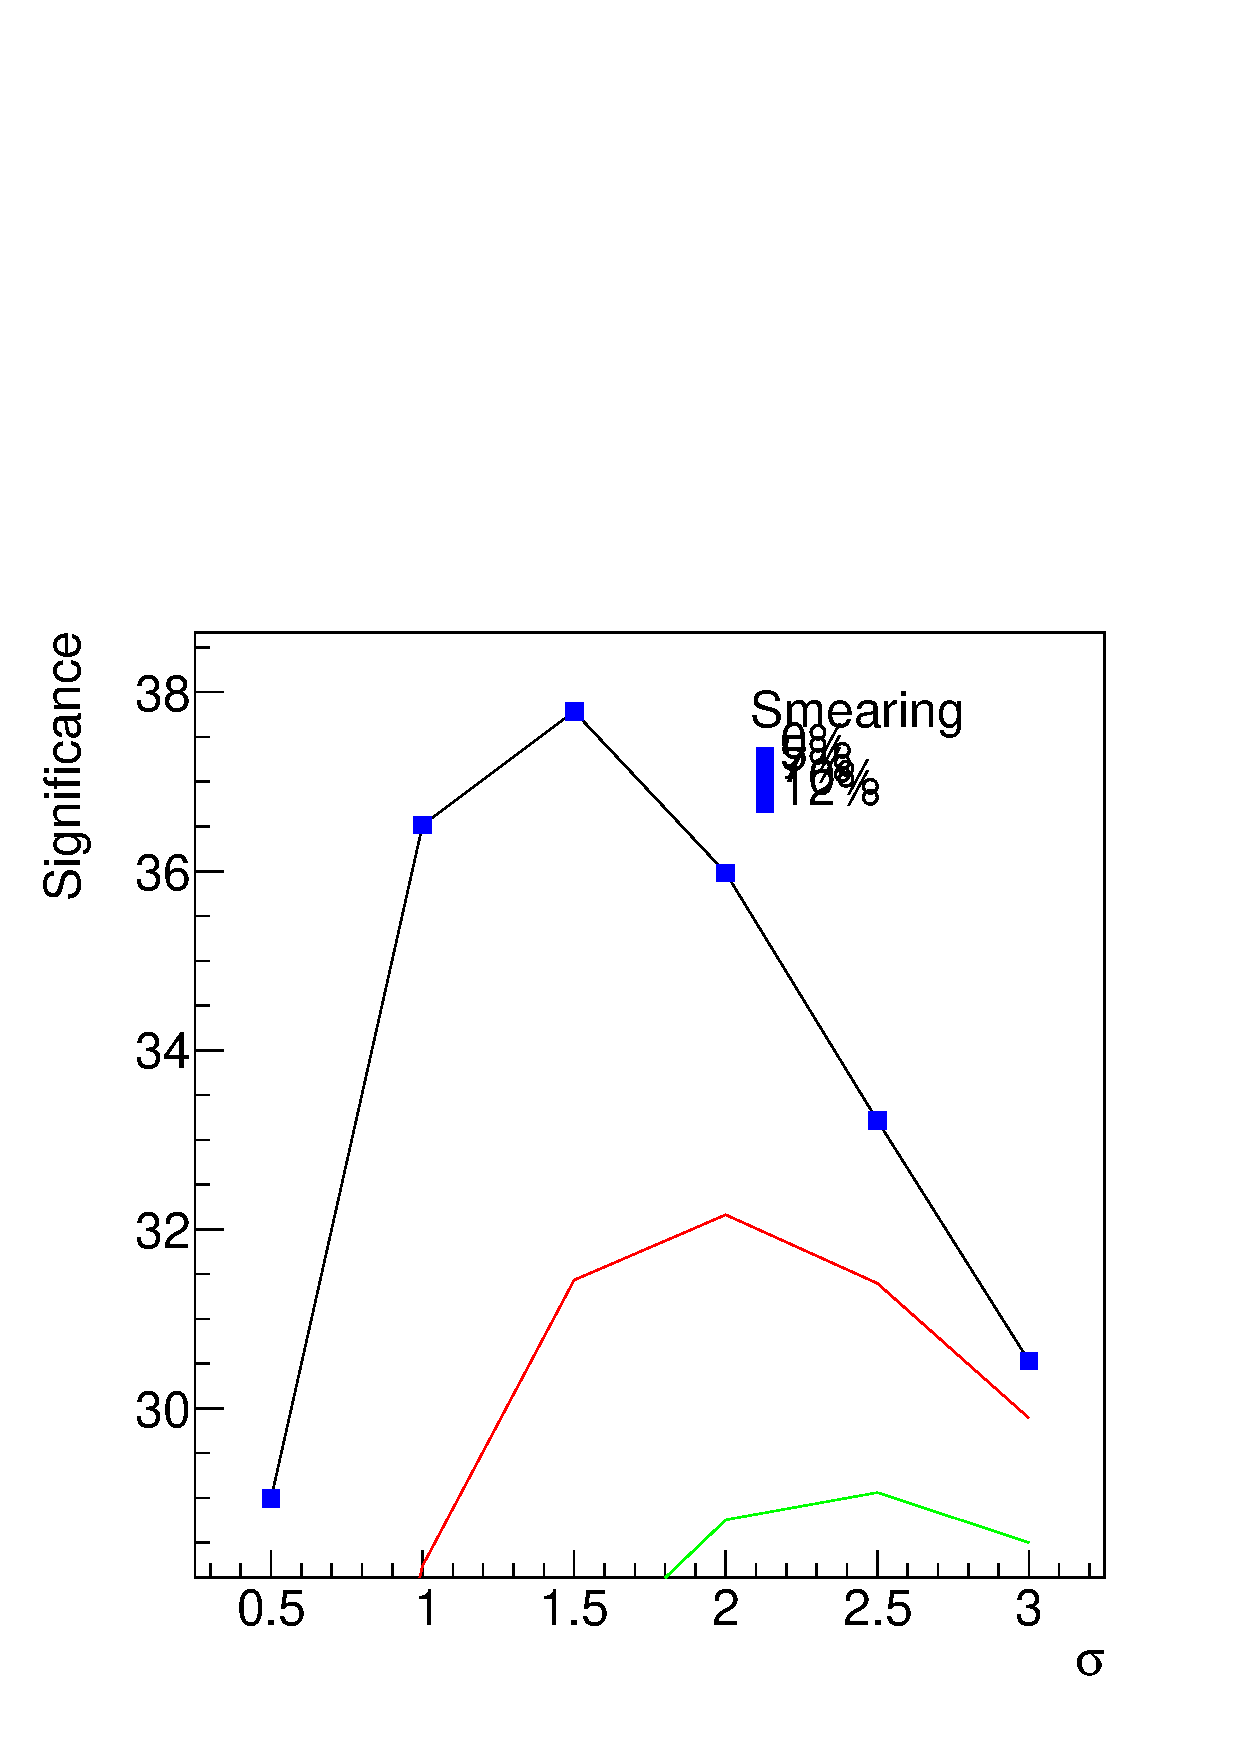
\includegraphics[page=1,width=\linewidth]{/home/kpapad/UG_thesis/Thesis/Bdt/src/WPhiJets_M60M5080_Significance.pdf}
\caption{}
\end{subfigure}
\caption{a: Summary of the ROC curves for the performance of the model on the data for each smearing case. b: Significances calculated across the BDT score range for the smearing cases of Table \ref{table:LightSmearings}. It is rather obvious that the perfomance of the classifier is the same for all the cases of smearing. }
\label{fig:LightROCSIG}
\end{figure}

\begin{table}[ht]
\centering
\begin{tabular}{|p{2cm}|p{3cm}|p{3cm}|}
 \hline
Smearing \%  & No. Sig. Events at BDT cut = 0.96 & No. Bkg.Events at BDT cut = 0.96 \\
\hline
0 & 1252 & 371 \\
5 & 912 & 371 \\
7 & 1235 & 371 \\
10 & 1246 & 371 \\
12 & 1243 & 371 \\
 \hline
\end{tabular}
\caption{Signal and background events at BDT cut 0.96 for different smearing percentages.}
\label{table:LightNumSIGBKG}
\end{table}

\begin{figure}[h!]
\centering
\includegraphics[page=2,width=0.5\textwidth]{/home/kpapad/UG_thesis/Thesis/Bdt/src/WPhiJets_M60M5080_Significance.pdf}
\caption{Evolution of significance for the smearing cases of table \ref{table:Smearings}. }
\label{fig:LightSigEvolBDT}
\end{figure}

\newpage
\subsection{Analysis Method II: Fit based analysis}
\label{sec:orgfec5bb4}
\label{sec:LightAnalysis_method2}
\subsubsection{Invariant mass reconstruction}
\label{sec:orgc57c22e}
\label{sec:Light_invariant_mass_reconstruction}
 The invariant mass spectrum is shown in Figure \ref{fig:LightAppMass}, and  is calculated using the features in Table \ref{table:DataSetFeatures}. 
\begin{figure}[h]
\centering
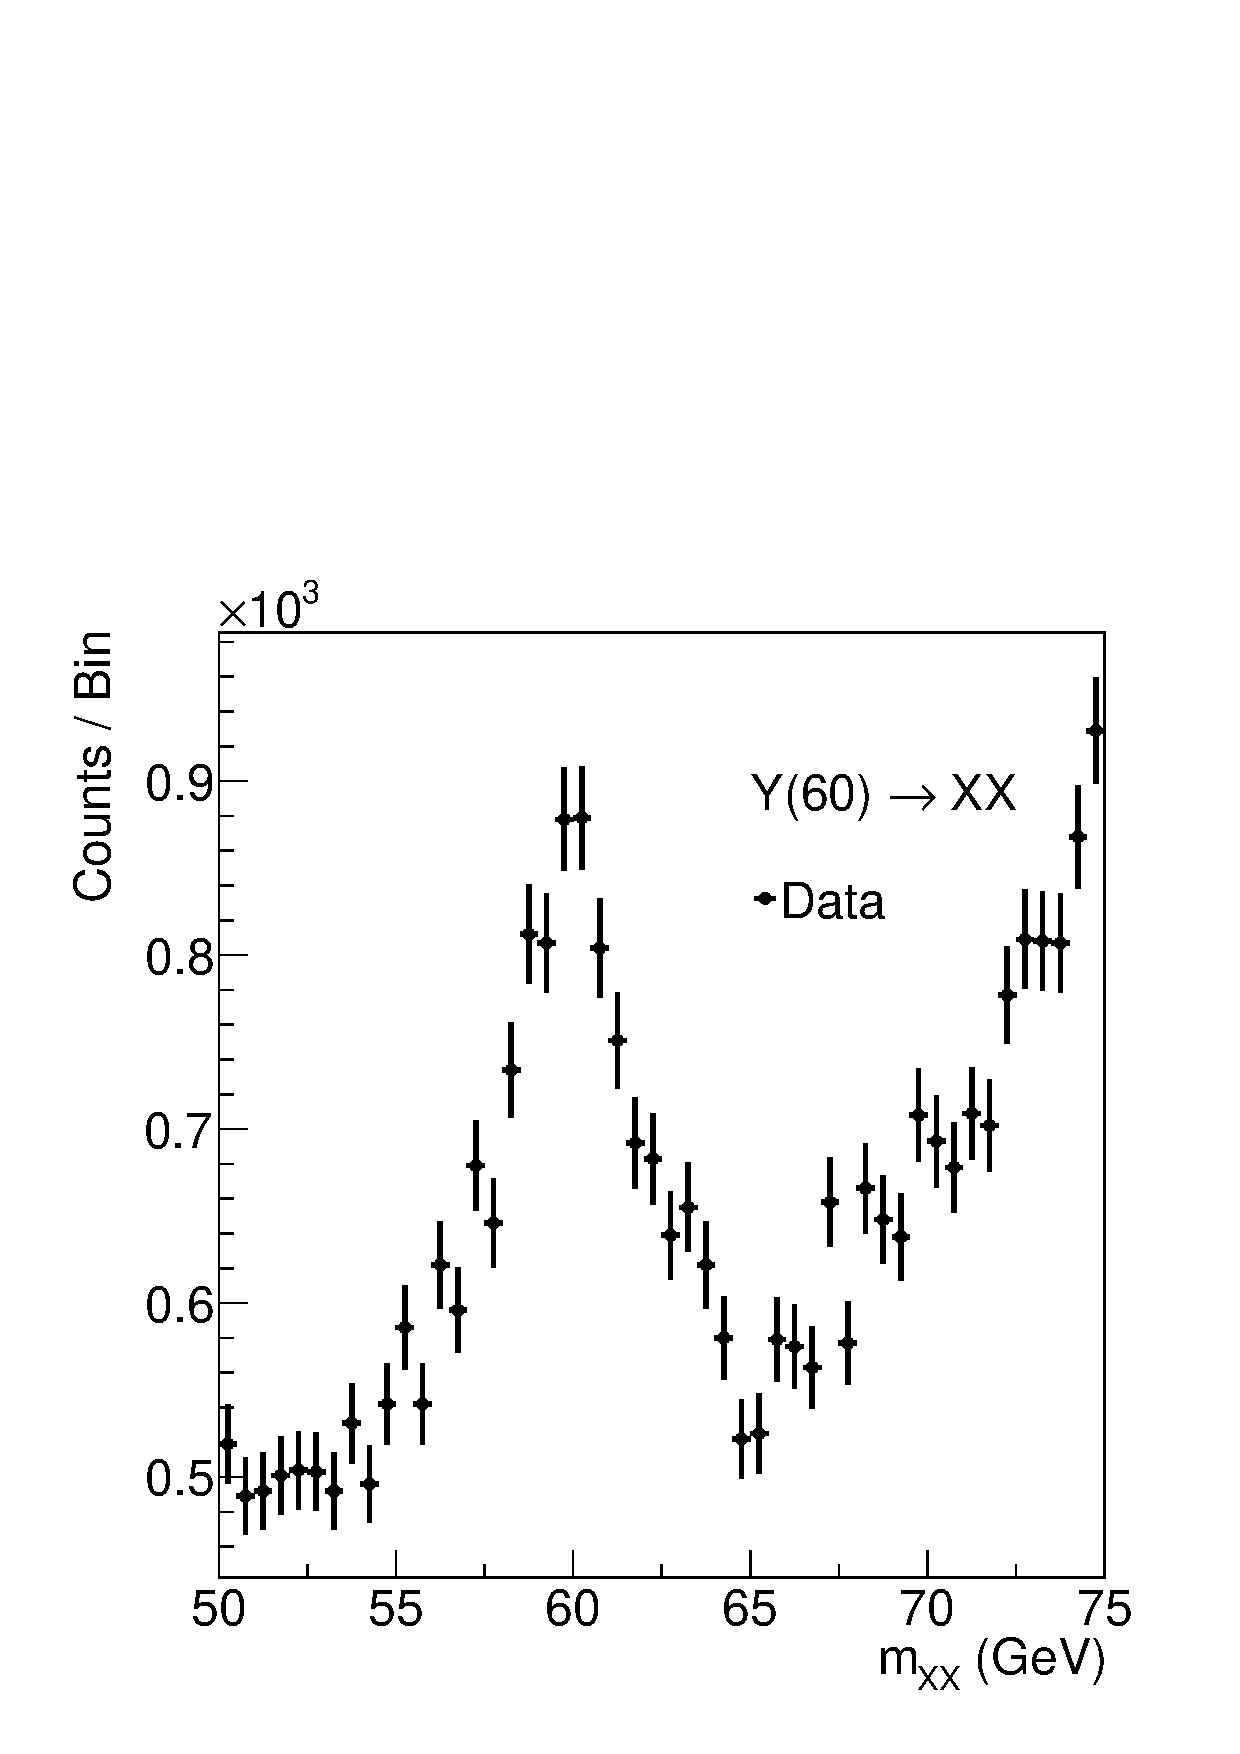
\includegraphics[page=1,width=0.5\textwidth]{/home/kpapad/UG_thesis/Thesis/Analysis/out/Plots/WPhiJets_M60M5080_Application_MassSpectrum.pdf}
\caption{The invariant mass spectrum of the application set}
\label{fig:LightAppMass}
\end{figure}

The reader may have noticed that the amount of signal present seems rather disproportionate to the amount of background. However, as discussed earlier, smearing has a significant effect on the present dataset due to low statistics. If it were not for the larger signal component, the invariant mass would have been completely smeared, even with very little smearing.
\subsubsection{Background Fitting}
\label{sec:orgb79b92a}
\label{sec:Light_background_fitting}
We proceed with fitting the mass, using the simplification discussed in section \ref{sec:Background_fitting}. That is, the background shape is fitted separately and kept constant throughout the signal fits.

The background shape is described by the function shown in Equation \ref{eq:LightbkgFitFunc}.
\begin{equation}
bkg(x) =  \alpha + \beta x + \gamma x^2 + \delta x^3,
\label{eq:LightbkgFitFunc}
\end{equation}
The parameters \(\alpha\), \(\beta\), \(\gamma\), and \(\delta\) are free parameters of the fit. The modeled background is illustrated in Figure \ref{fig:LightBKGfit}.
\begin{figure}[h]
\centering
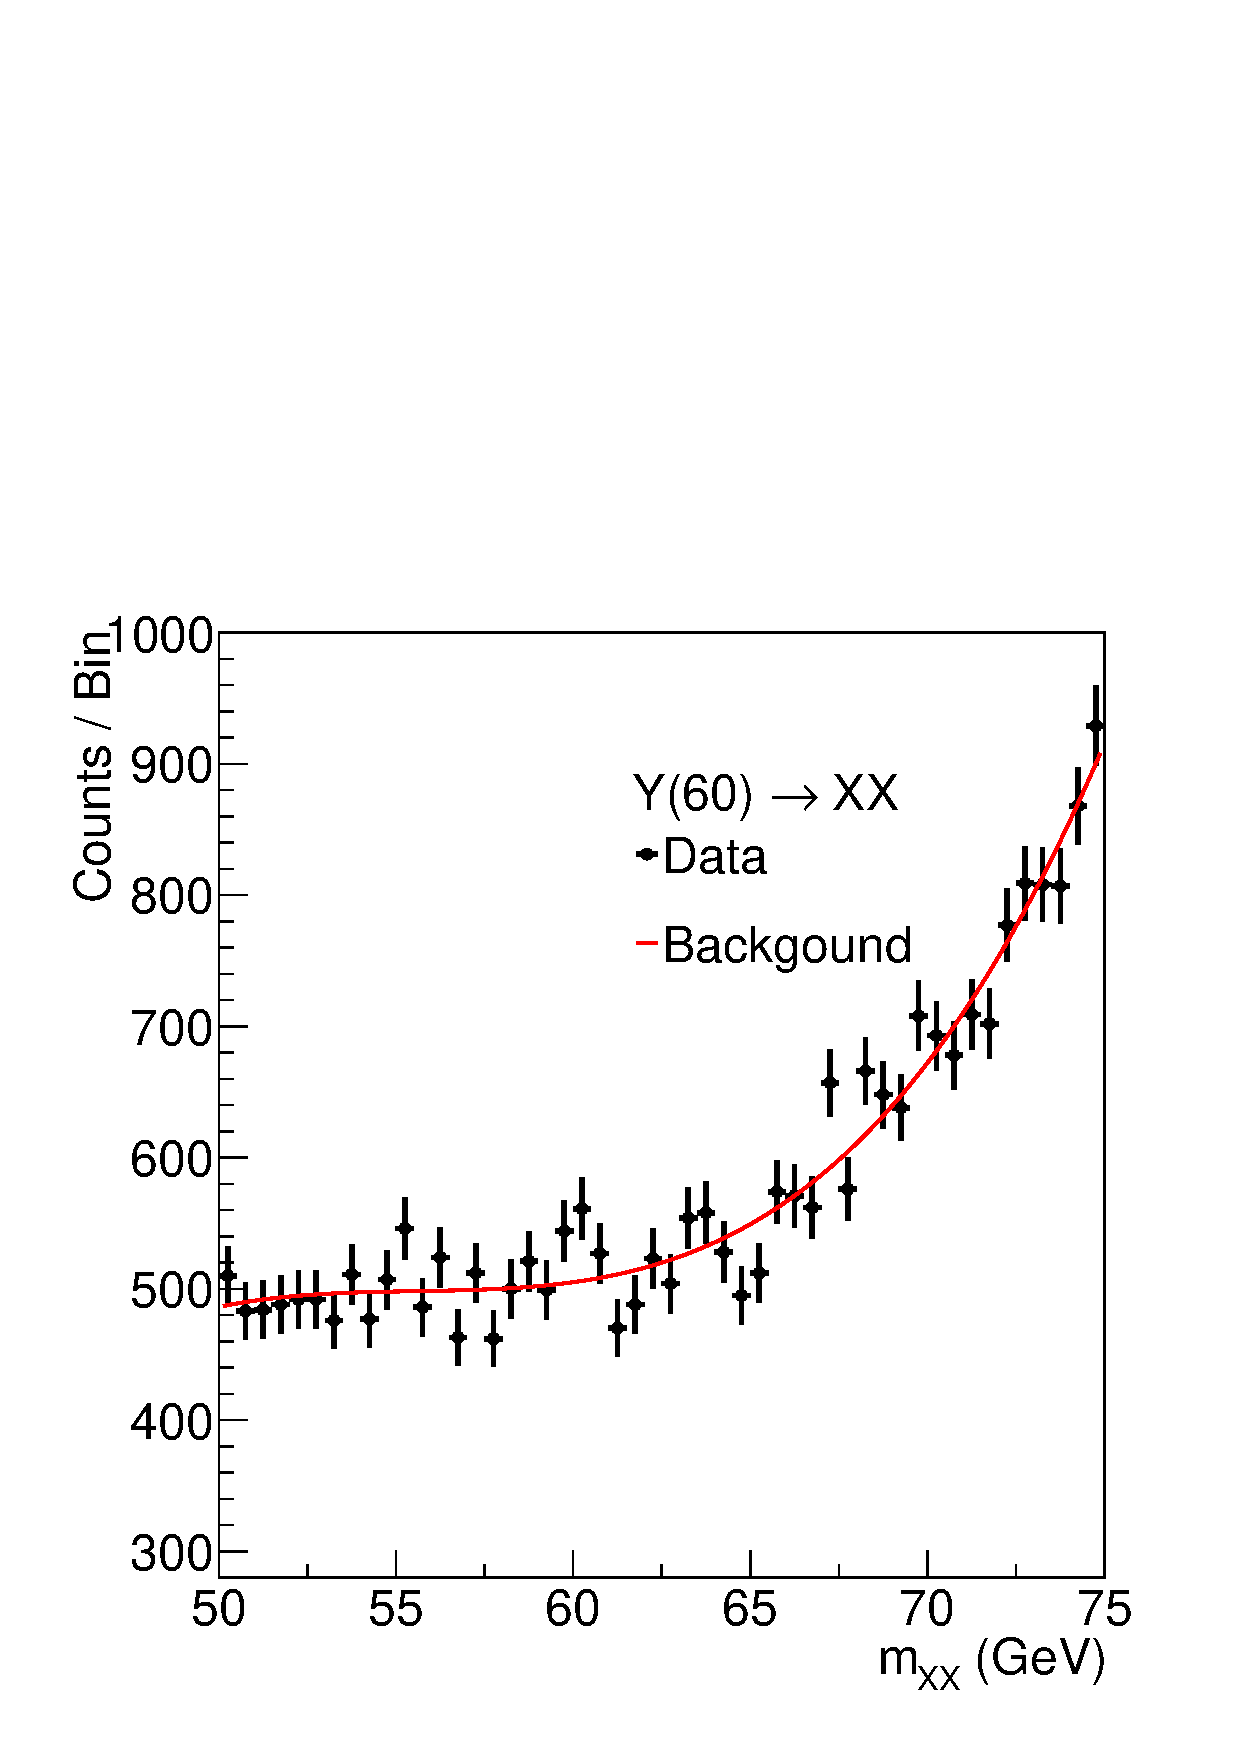
\includegraphics[page=1,width=0.5\textwidth]{/home/kpapad/UG_thesis/Thesis/Analysis/out/Plots/WPhiJets_M60M5080_Application_bkgonly_Fit.pdf}
\caption{The fitted background}
\label{fig:LightBKGfit}
\end{figure}
\subsubsection{Signal Fitting}
\label{sec:orgf4b823b}
\label{sec:Light_signal_fitting}
To fit the signal, a Gaussian function with \(\sigma\) and magnitude as free parameters, and \(\mu = 60\text{GeV}\), is used. Figure \ref{fig:Lightfits} shows the fitted invariant mass spectra for smearing percentages of \(0\%\), \(5\%\), \(7\%\), \(10\%\), and \(12\%\). As shown in Figure \ref{fig:Lightfits}, smearing cases above \(12\%\) would completely smear the signal component, and the fit analysis method would have failed.
\subsubsection{Signal from background separation}
\label{sec:org073f9f1}
\label{sec:Light_signal_from_background_separation}
The signal from the background separation process in this study is the same as that in section \ref{sec:Signal_from_background_separation}. We scan various mass windows around the center of the signal to find the region that yields the best significance. Moving with a step of \(0.5\sigma\), we scanned six different regions from \(\pm 0.5\sigma\) up to \(\pm 3\sigma\). Looking at the results in figure \ref{fig:LightScan0}, the region \(\pm 1.5\sigma\) provides the best performance in terms of significance.
\begin{figure}[h]
\centering
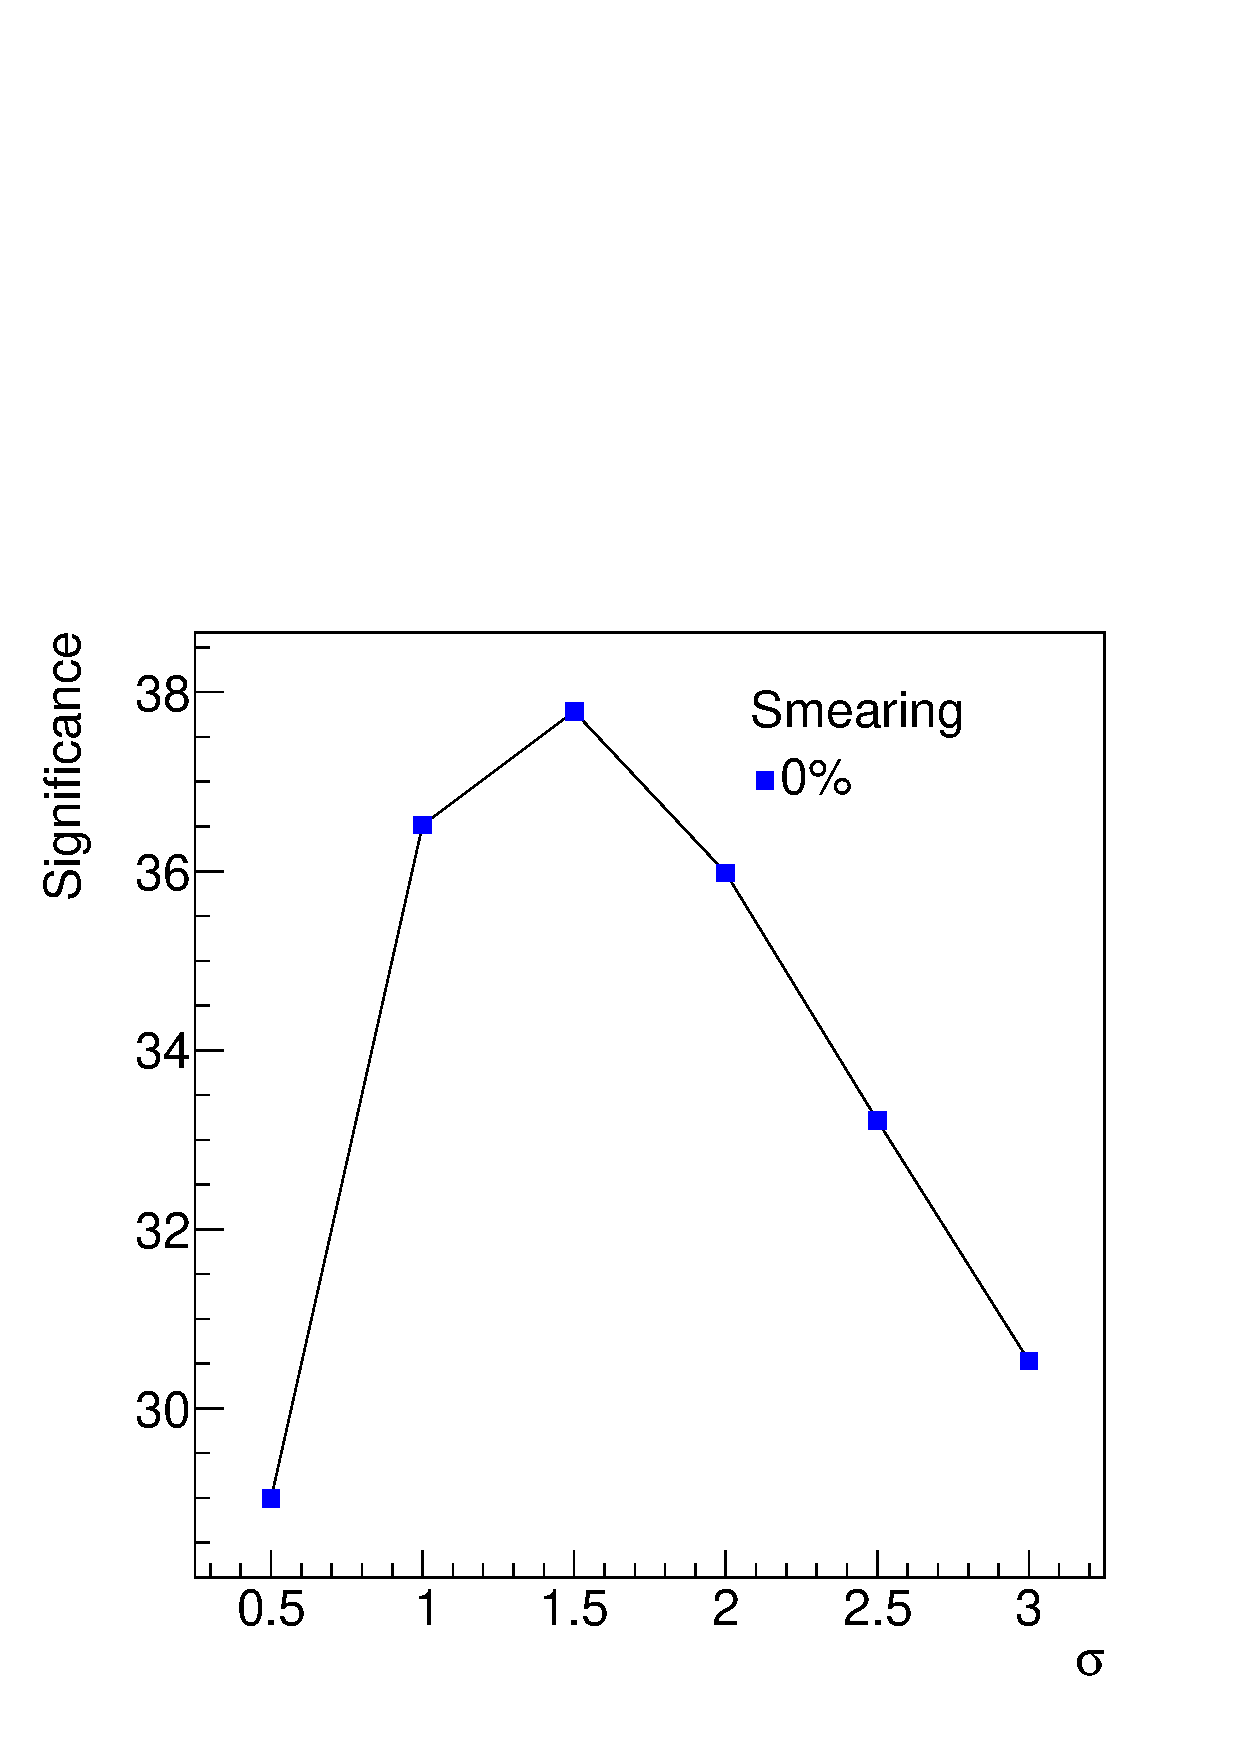
\includegraphics[page=1,width=0.5\textwidth]{/home/kpapad/UG_thesis/Thesis/Analysis/src/WPhiJets_M60M5080_Significance0.pdf}
\caption{Scan of significance for various values of $\sigma$, in the $0\%$ smearing case. We see that the regrion $\pm 1.5\sigma$ around $\mu=60GeV$, gives the best significance.}
\label{fig:LightScan0}
\end{figure}

We study the changes in significance as a function of smearing, in the fixed window and adaptive window interpretations discussed in section \ref{sec:Signal_from_background_separation}. The actual values of \(\sigma\), and the corresponding mass window for the adaptive window search, are summarized in table \ref{table:LightAdaSigmas}. The results are presented in Figure \ref{fig:LightAdaFixedSig}, and Table \ref{table:LightNumSigBkg}, which summarizes the amount of signal and background events present in the region of interest for both studies (fixed and adaptive window).
\begin{figure}[h]
\centering
\includegraphics[page=3,width=0.5\textwidth]{/home/kpapad/UG_thesis/Thesis/Bdt/src/WPhiJets_M60M5080_Significance.pdf}
\caption{Copmarison of the significance evolution as caclulated in the fixed widow and adaptive window case.} 
\label{fig:LightAdaFixedSig}
\end{figure}

\begin{table}[h]
\centering
\begin{tabular}{|p{2cm}|p{2cm}|c|}
 \hline
Smearing \%  & $\sigma$ in GeV & Invarian Mass $\pm 1.5\sigma$ window  in GeV \\
\hline
0 & 2.1267 & 6.38 \\
5 & 2.9933 & 8.98 \\
7 & 3.6933 & 11.08 \\
10 & 4.84 & 14.52 \\
12 & 5.5133 & 16.54 \\
 \hline
\end{tabular}
\caption{Summary of the invariant mass windows used used in adapitve window study. Note that the resulting window of $0\%$ smearing corresponds to the fixed window case as well.}
\label{table:LightAdaSigmas}
\end{table}

\begin{table}[h!]
\centering
\begin{tabular}{|p{2cm}|p{3cm}|p{3cm}|p{3cm}|p{3cm}|}
 \hline
Smearing \%  & No. Sig. Events (fixed window) & No. Bkg.Events (fixed window) & No. Sig. Events (adaptive window) & No. Bkg.Events (adaptive window)  \\
\hline
0 & 3040 & 6474 & 3040 & 6474 \\
5 & 2529 & 6474 & 3069 & 9150 \\
7 & 2183 & 6474 & 3091 & 11364 \\
10 & 1770 & 6474 & 3131 & 15049 \\
12 & 1553 & 6474 & 3080 & 17263 \\
 \hline
\end{tabular}
\caption{Signal and background events in the 6.38Gev fixed window region and in the $\pm 1.5\sigma$ adaptive window region, for different smearing percentages.}
\label{table:LightNumSigBkg}
\end{table}

\subsection{Results}
\label{sec:orgf65369b}
The study of multivariate and single variate classification techniques in a signal from background separation task, in the lower mass region, returned interesting results, which are going to be discussed in the present section. 
\begin{figure}[h]
\centering
\includegraphics[page=4,width=0.5\textwidth]{/home/kpapad/UG_thesis/Thesis/Bdt/src/WPhiJets_M60M5080_Significance.pdf}
\caption{ Comparison of the perfomance of the BDT and Fit based analysis, in terms of sifnificance,  as a function of the smearing cases. We can see that BDT based analysis, is more robust.}
\label{fig:LightBdtFitSig}
\end{figure}

A comparison between the significance yielded by each method, as a function of smearing, is presented in Figure \ref{fig:LightBdtFitSig}. What is striking is the performance, in terms of significance, of the two methods. It is evident that the BDT classifier provides the best performance, while being more or less unaffected by energy scale uncertainties. To further investigate this compelling result, we can take a look at the model's feature importance (a score that indicates how useful or valuable each feature was in the construction of the boosted decision trees within the model), presented in Figure \ref{fig:LightFeatureImportance}. Even though the actual meaning of the score is different depending on the training algorithm, the feature whose role is the most significant in the classification task, is the \(\Delta\phi\) of the particles, a variable that as already mentioned, is not affected by smearing.

On the other hand, the performance of the fit model is similar to that of the heavy mass search. The significance it returns drops as the invariant mass smearing percentage increases, until it reaches a "breaking point".
\begin{figure}[h!]
\centering
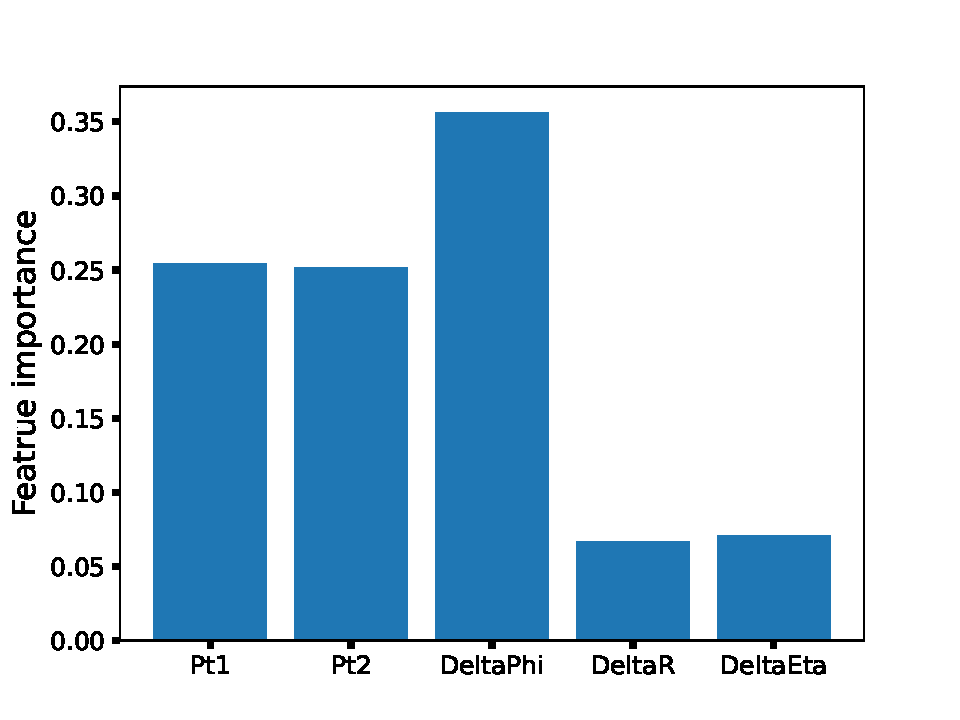
\includegraphics[page=1,width=0.5\textwidth]{/home/kpapad/UG_thesis/Thesis/Bdt/out/Plots/feature_importance_lm.pdf}
\caption{The feature importance of the BDT classifier. The model's performance on smeared data is rather stable, due to its strong dependance on $\Delta\phi$, a variable that remains invariant under smearing. }
\label{fig:LightFeatureImportance}
\end{figure}


\begin{figure}[hp]
\centering
\begin{subfigure}{0.45\textwidth}
\centering
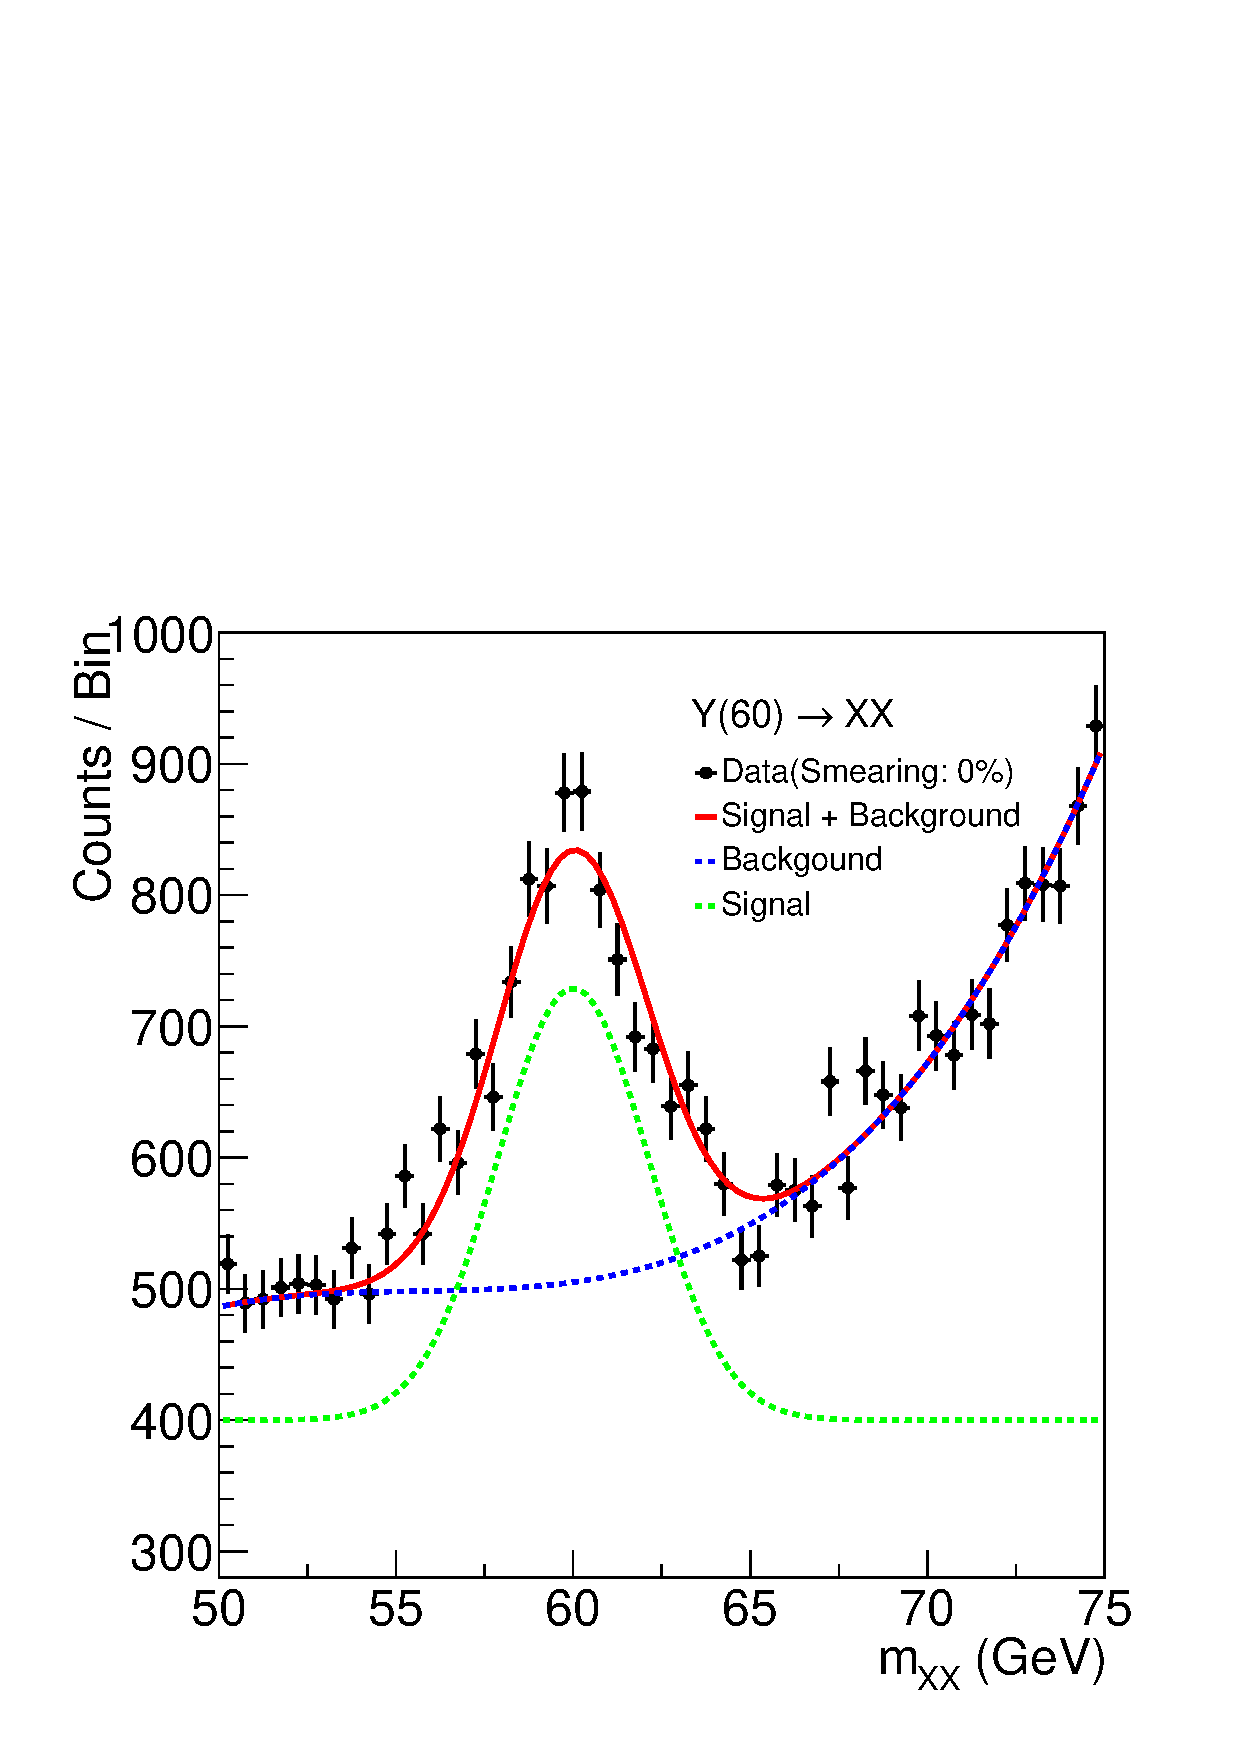
\includegraphics[page=1,width=\linewidth]{/home/kpapad/UG_thesis/Thesis/Analysis/src/WPhiJets_M60M5080_FitALL.pdf}
\caption{}
\end{subfigure}
\begin{subfigure}{0.45\textwidth}
\centering
\includegraphics[page=2,width=\linewidth]{/home/kpapad/UG_thesis/Thesis/Analysis/src/WPhiJets_M60M5080_FitALL.pdf}
\caption{}
\end{subfigure}

\begin{subfigure}{0.45\textwidth}
\centering
\includegraphics[page=3,width=\linewidth]{/home/kpapad/UG_thesis/Thesis/Analysis/src/WPhiJets_M60M5080_FitALL.pdf}
\caption{}
\end{subfigure}
\begin{subfigure}{0.45\textwidth}
\centering
\includegraphics[page=4,width=\linewidth]{/home/kpapad/UG_thesis/Thesis/Analysis/src/WPhiJets_M60M5080_FitALL.pdf}
\caption{}
\end{subfigure}

\begin{subfigure}{0.45\textwidth}
\centering
\includegraphics[page=5,width=\linewidth]{/home/kpapad/UG_thesis/Thesis/Analysis/src/WPhiJets_M60M5080_FitALL.pdf}
\caption{}
\end{subfigure}
\caption{Fits for the following smearing cases a: $0\%$, b: $5\%$, c: $7\%$, d: $10\%$, e: $12\%$}
\label{fig:Lightfits}
\end{figure}
